% Overleaf: set the compiler to pdfLaTeX (Menu > Settings > Compiler) and the
% main document to main.tex. Bibliography: BibTeX with refs.bib.
\documentclass[journal]{IEEEtran}

\usepackage{cite}
\usepackage{amsmath,amssymb}
\usepackage{graphicx}
\usepackage{booktabs}
\usepackage{multirow}
\usepackage{array}
\usepackage{algorithm}
\usepackage{algpseudocode}
\usepackage{url}
\usepackage{xcolor}
\usepackage[hidelinks]{hyperref}

\graphicspath{{figures/}}

% Placeholders that must be filled before submission are shown in red.
\newcommand{\fillin}[1]{\textcolor{red}{[#1]}}
\newcommand{\F}{F}                 % every run failed
\newcommand{\na}{--}               % not run in this test
\newcommand{\pc}[1]{$#1$}          % signed percentage in a table cell

\begin{document}

\title{Does Learning Help Oxygen Control on BSM1?\\
A Reproduction of Multiagent Adaptive Critic Control\\
With Pre-Registered Held-Out Tests}

\author{Amritha~\fillin{surname},~\fillin{supervisor name}%
\thanks{\fillin{Affiliation, department, city, country. E-mail.}}%
\thanks{Code, results and the pre-registration commits:
\url{https://github.com/Amritha902/water_resource}.}}

\markboth{\fillin{Journal name}}{Amritha \MakeLowercase{\textit{et al.}}: Does Learning Help Oxygen Control on BSM1?}

\maketitle

\begin{abstract}
A recent paper reported that a multiagent adaptive critic controller (MAACC)
built on a PID prior cuts the dissolved-oxygen tracking error of the Benchmark
Simulation Model No.~1 (BSM1) by 92--95\,\% relative to that PID. We rebuilt
the controller from its printed equations and parameters on the official BSM1
code. Our PID matches the published oxygen error within 1\,\% in dry and storm
weather and within 10\,\% in rain, but MAACC as printed stays equal to its PID
in 80 of 80 runs. With standard off-policy training (replay, twin target
critics, delayed actor updates) the same architecture does learn: $-85$\,\%
in dry weather on a test week it never saw. A PID whose P and I gains are
tuned per loop, with a daily iterative learning controller (ILC) added,
reaches $-90/-89/-80$\,\% (dry/rain/storm) without any neural network, and a
soft actor-critic trained by imitation and placed on top of it adds nothing
measurable. We then ran two held-out tests whose protocols were committed
before any run: influent windows from BSM2 and the official BSM1 sensor
models. Under the official sensor noise every high-gain controller, learned
or not, either failed or lost its advantage, and no controller we tested
beat the original PID there. The most useful changes we found were not
learned: an anti-windup rule for the ILC ($-39$\,\% error under overload
with ideal sensors) and a filtered, lower-gain variant that finished every
held-out run but did not beat the original PID under sensor noise. All
76 checks of a final audit of the reported numbers pass.
\end{abstract}

\begin{IEEEkeywords}
Wastewater treatment, BSM1, dissolved oxygen control, reinforcement
learning, adaptive critic, iterative learning control, reproducibility,
pre-registration.
\end{IEEEkeywords}

%=====================================================================
\section{Introduction}
%=====================================================================

\IEEEPARstart{A}{eration} is where most of the electricity of an
activated-sludge plant goes, and the dissolved-oxygen (DO) loop that sets it
is the first loop any control study of such a plant looks at. The Benchmark
Simulation Model No.~1 (BSM1)~\cite{alex2008bsm1,gernaey2014benchmarking}
gives the field a shared plant, shared influent files and shared
performance measures, so results from different groups can in principle be
compared directly.

Several recent papers control BSM1 with learning controllers that start from
a PID and learn a correction on top of it~\cite{wang2026maacc,du2023do,zhao2025ioql}.
The gains reported are large. Wang \emph{et al.}~\cite{wang2026maacc}
propose a multiagent adaptive critic controller (MAACC) with one agent per
loop and an incremental PID as expert knowledge, and report oxygen tracking
errors 95, 95 and 92\,\% lower than the PID in dry, rain and storm weather.

Two things make such numbers hard to interpret. The first is the baseline:
a PID with the gains used in the paper is one tuning among many, and a gain
reduction against a weakly tuned PID says little about the value of
learning. The second is the test: the standard BSM1 evaluation uses ideal
sensors and three influent files that a controller can be tuned against.
Both concerns are familiar from the reinforcement-learning literature, where
results are known to depend on seeds, baselines and evaluation
details~\cite{henderson2018matters,pineau2021reproducibility}.

This paper reports what happened when we tried to reproduce MAACC and to
improve on it, on the official BSM1 code~\cite{bsm2python}, under a
protocol designed to make the comparison hard to fool. Our contributions are:
\begin{enumerate}
\item A reimplementation of MAACC from the printed equations and Table~I of
  \cite{wang2026maacc}. The plant and PID reproduce the paper's PID numbers;
  the learned controller does not learn as printed, and we show why.
\item A repaired MAACC that keeps the paper's architecture and replaces its
  training with standard off-policy tools~\cite{fujimoto2018td3,ackermann2019matd3}.
  It learns.
\item Stronger non-learned baselines: a PID tuned term by term with a fixed
  stability margin, and a daily ILC with bumpless transfer and anti-windup.
  On the nominal test this matches or beats every learned controller,
  including a soft actor-critic with imitation learning (SAC-IL) that we
  designed for the purpose.
\item Two held-out tests with seven conditions, each protocol committed to a
  public repository before its first run~\cite{nosek2018prereg}. They show
  that sensor noise, not tracking accuracy, is the binding constraint.
\item An audit of every reported number (76 of 76 checks pass), and the full
  code and result files.
\end{enumerate}

The short version is that learning was not where the improvement came from.
Most of it came from tuning and from exploiting the daily repetition of the
load, and none of it survived the official sensor noise intact.

%=====================================================================
\section{Related Work}
%=====================================================================

\emph{Benchmarks.} BSM1~\cite{alex2008bsm1} couples five ASM1~\cite{henze2000asm}
reactors with a ten-layer settler and defines influent files, sensor and
actuator models and evaluation criteria. BSM2~\cite{jeppsson2007bsm2} extends
it to a full plant with a 609-day influent that includes seasonal and weekly
variation. We use the Python implementation \texttt{bsm2-python}~\cite{bsm2python}.

\emph{Learning control on BSM1.} Adaptive critic designs belong to the
adaptive dynamic programming family~\cite{lewis2009adp}. Wang \emph{et al.}
use one per loop with a centralized critic input and a PID prior~\cite{wang2026maacc};
Zhao \emph{et al.} integrate online Q-learning with a PID~\cite{zhao2025ioql};
Du \emph{et al.} use deep reinforcement learning to let the oxygen set point
float~\cite{du2023do}. On the deep reinforcement learning side, we use the
twin-critic and delayed-update ideas of TD3~\cite{fujimoto2018td3}, their
multiagent form~\cite{lowe2017maddpg,ackermann2019matd3}, soft
actor-critic~\cite{haarnoja2018sac}, and an imitation term kept above a floor
as in TD3+BC~\cite{fujimoto2021td3bc}.

\emph{Iterative learning control.} ILC improves a repeated task from one
trial to the next~\cite{arimoto1984ilc,bristow2006ilc}. A plant load that
repeats every day is such a task, with the day as the trial. Our update,
which learns a feedforward from the correction the feedback controller had
to make, is close to feedback-error learning~\cite{gomi1993fel}.

%=====================================================================
\section{Plant, Task and Measures}
%=====================================================================

\begin{figure}[!t]
\centering
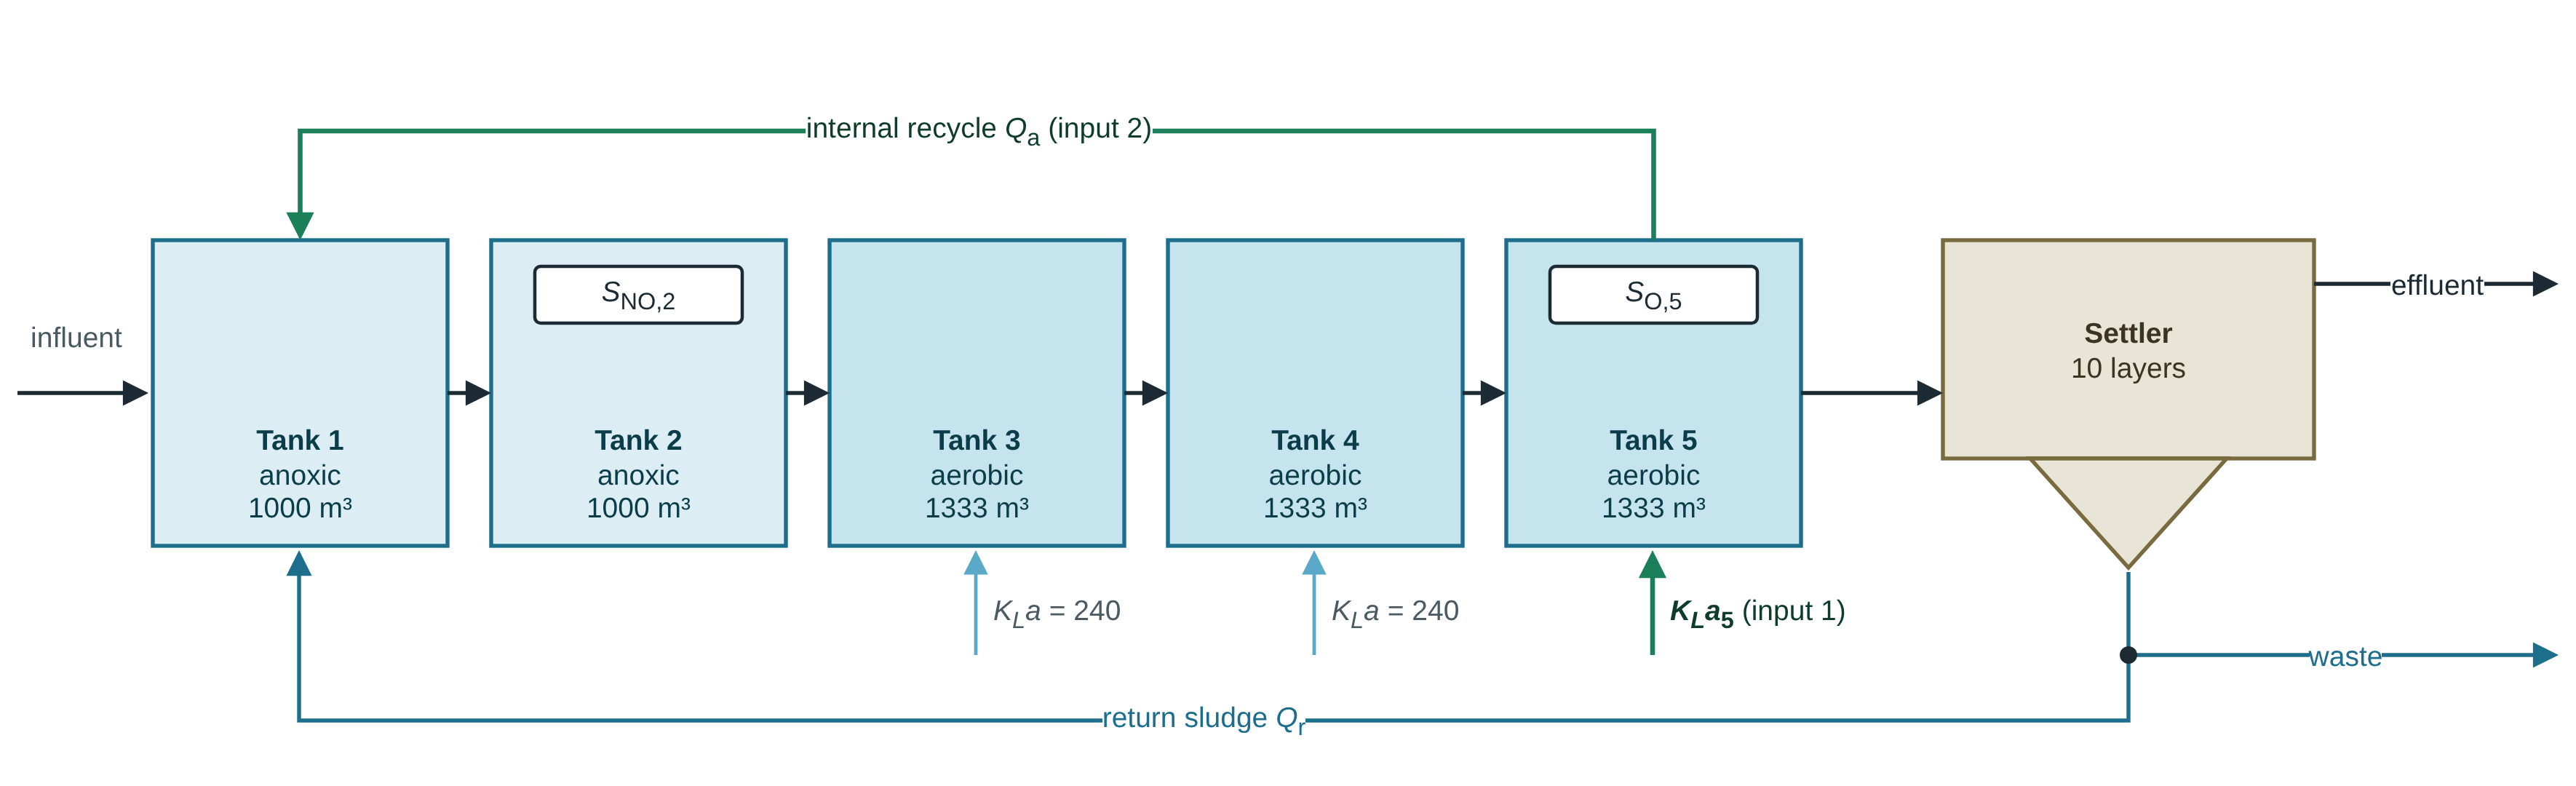
\includegraphics[width=\columnwidth]{d0_plant}
\caption{BSM1 and the two loops of~\cite{wang2026maacc}. Oxygen in tank~5
is controlled through the aeration $K_La_{,5}$; nitrate in tank~2 through
the internal recycle $Q_a$.}
\label{fig:plant}
\end{figure}

\subsection{Plant and loops}
BSM1 has two anoxic tanks of 1000\,m$^3$, three aerated tanks of
1333\,m$^3$ and a secondary settler (Fig.~\ref{fig:plant}). As
in~\cite{wang2026maacc}, two loops are closed:
\begin{itemize}
\item oxygen: $S_{O,5}\to 2$\,mg/L through $K_La_{,5}\in[0,240]$\,d$^{-1}$;
\item nitrate: $S_{NO,2}\to 1$\,mg/L through $Q_a\in[0,92\,230]$\,m$^3$/d.
\end{itemize}
The control period is 45\,s. $K_La$ of tanks 3 and 4 is fixed at
240\,d$^{-1}$. The paper prints the set points as $[1,2]$; its figures and
PID errors only match the standard BSM1 values $[2,1]$, which we use.

\subsection{Influent and initial state}
We use the official 14-day dry, rain and storm files (15-min samples).
In the spreadsheet versions of the rain and storm files the inert soluble
COD $S_I$ is 30\,g/m$^3$ in every row; in the official data it is diluted
by the rain, $S_I = 30\,Q_\text{dry}/Q$, and we apply this correction.
$S_I$ is inert, so it affects effluent COD only. Every run starts from the
state reached after 14 days of dry weather under the paper's PID.

\subsection{PID prior}
The paper's PID is incremental:
\begin{equation}
\Delta u_k = K_p(e_k-e_{k-1}) + K_i e_k + K_d(e_k-2e_{k-1}+e_{k-2}),
\label{eq:pid}
\end{equation}
with $e = r-y$, $K_p=\mathrm{diag}\{100,10^5\}$,
$K_i=\mathrm{diag}\{20,3\times10^4\}$ and $K_d=\mathrm{diag}\{10,10^3\}$,
the first entry for oxygen and the second for nitrate.

\subsection{Measures}
Following~\cite[eq.~(36)]{wang2026maacc}, for each loop
\begin{equation}
\mathrm{IAE}=\frac1N\sum_{k=1}^N|e_k|,\quad
\mathrm{ISE}=\frac1N\sum_{k=1}^N e_k^2,\quad
\mathrm{DEV}_{\max}=\max_k|e_k|.
\end{equation}
Errors are always computed from the true concentrations, not the measured
ones. We also report the aeration movement $\sum_k|K_La_{,5}(k)-K_La_{,5}(k-1)|$
per day, aeration energy and effluent quality. A run in which $S_{O,5}$
leaves $[0.3,4]$\,mg/L is stopped and counted as a \emph{failure}; this rule
is ours, not the paper's.

%=====================================================================
\section{Reproducing MAACC}
%=====================================================================

\begin{figure*}[!t]
\centering
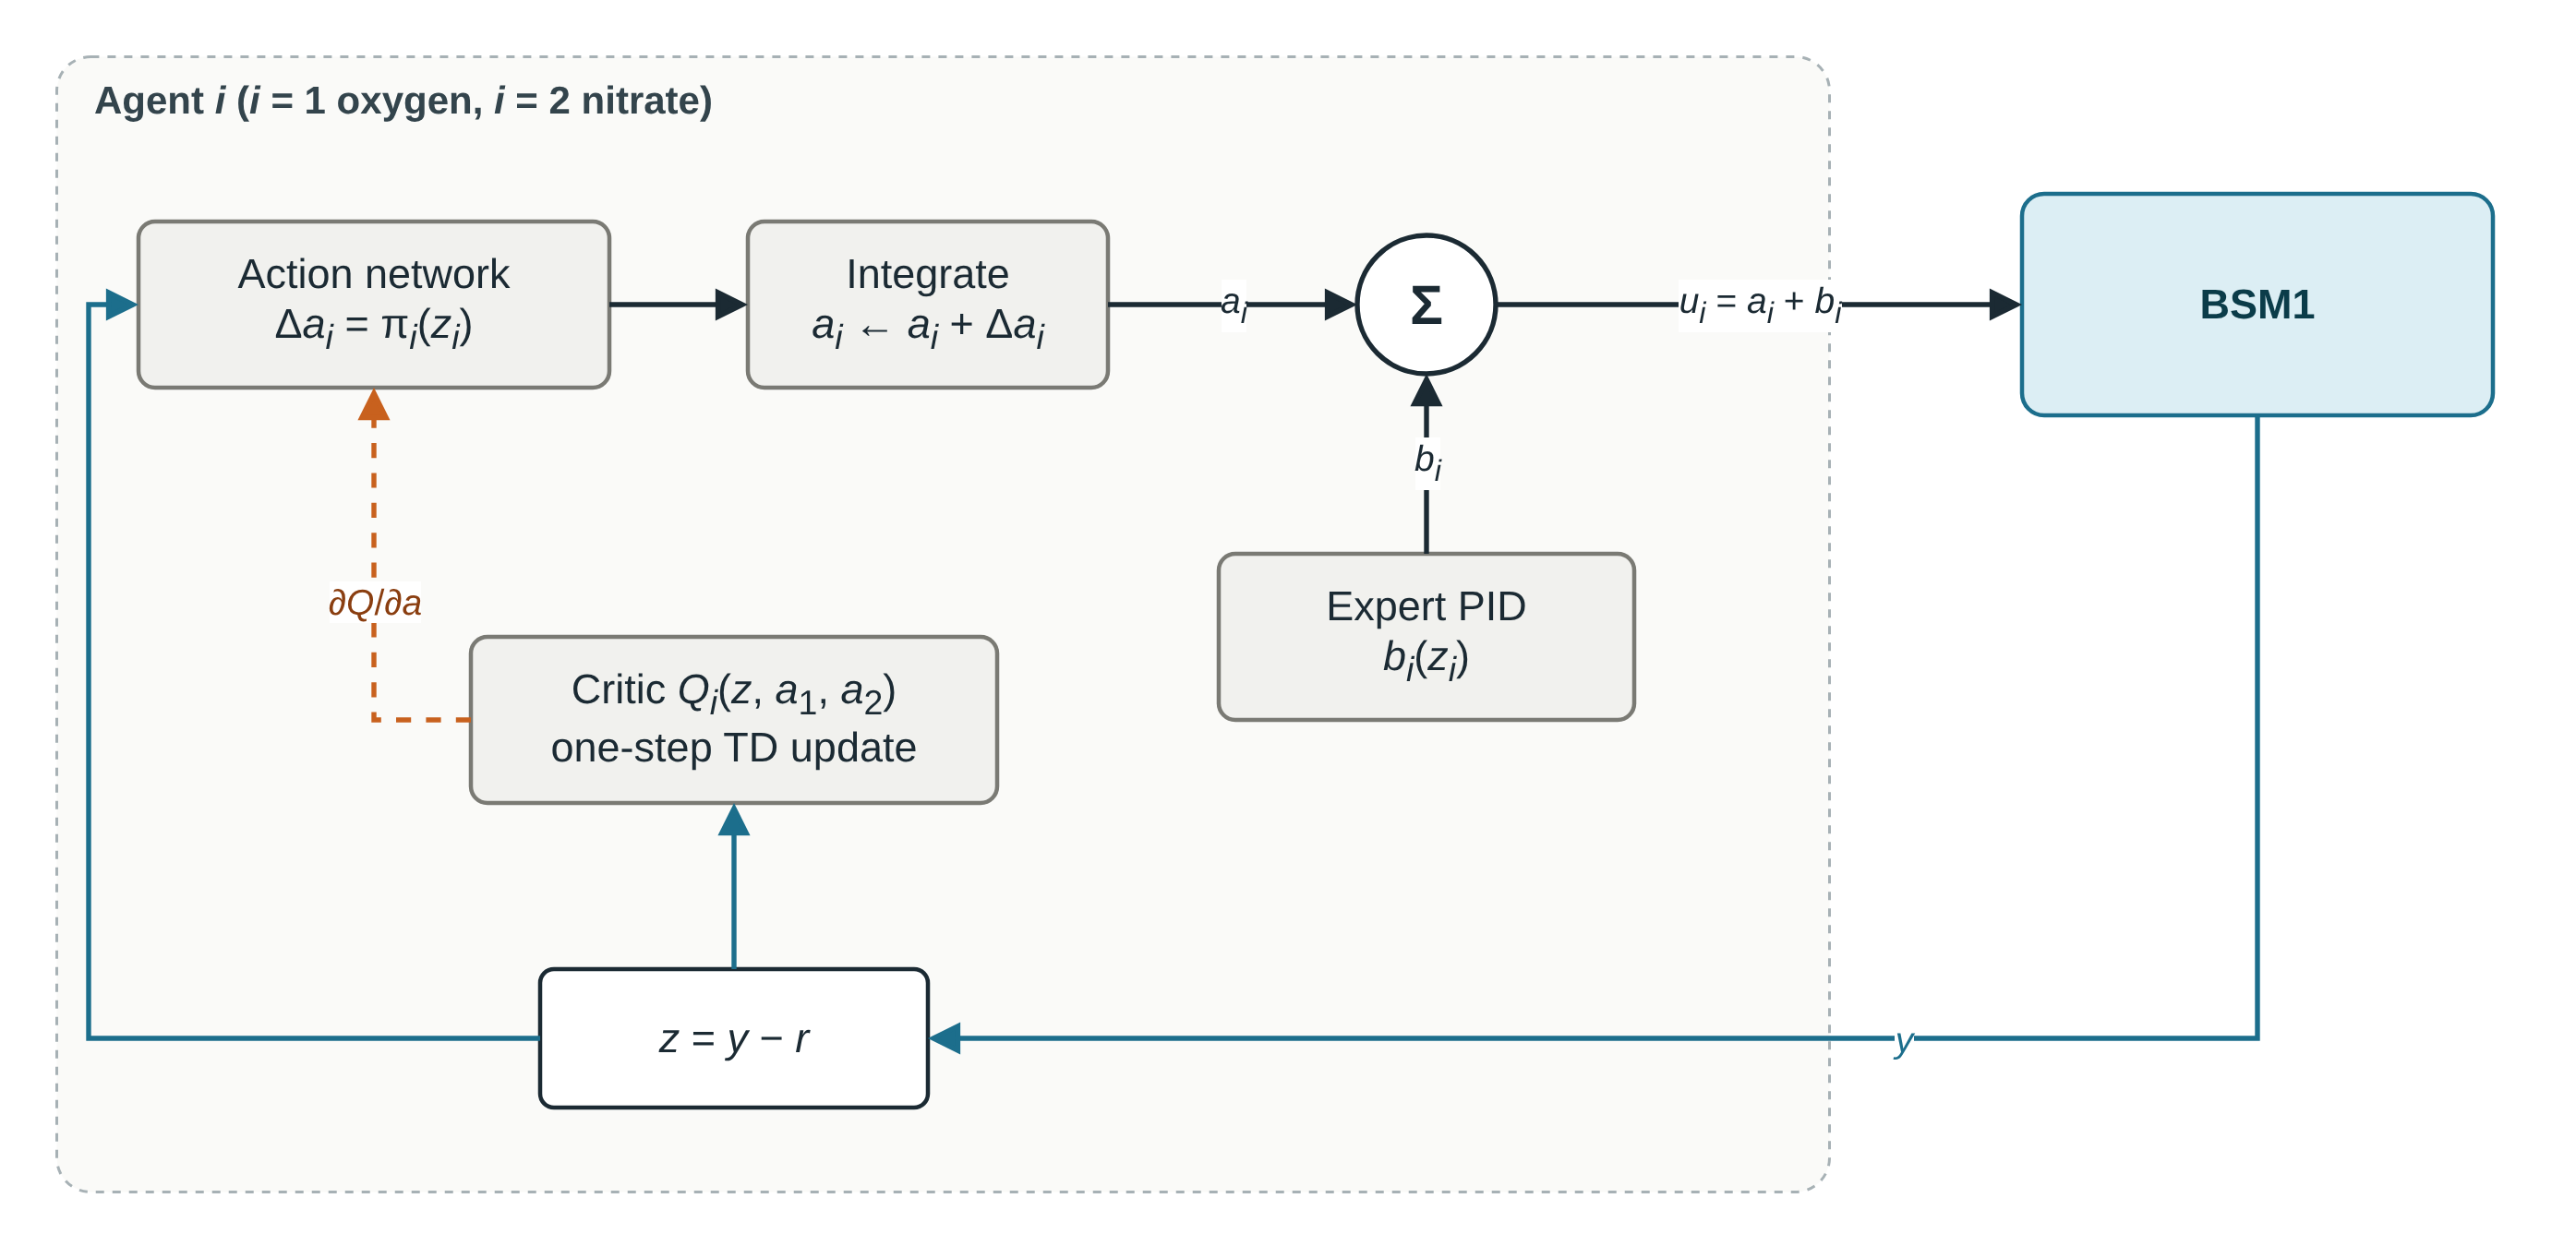
\includegraphics[width=0.72\textwidth]{d1_paper}
\caption{MAACC as described in~\cite{wang2026maacc}. One agent is drawn;
the oxygen and nitrate agents have the same form and are coupled through
their critics, which see both loops and both actions. The action network
outputs an increment, which is integrated and added to the PID output,
$u_i=a_i+b_i$. Each sample is used once, in a one-step temporal-difference
update (dashed).}
\label{fig:maacc}
\end{figure*}

We implemented every equation of~\cite{wang2026maacc} and every weight and
learning rate of its Table~I (Fig.~\ref{fig:maacc}) and ran 20 runs per case
(dry, rain, storm, dry with actuator noise). Table~\ref{tab:repro} compares
the 14-day oxygen IAE with the paper's Table~II.

\begin{table}[!t]
\centering
\caption{Oxygen IAE over 14 days: published values and our runs.}
\label{tab:repro}
\begin{tabular}{lccc}
\toprule
 & Dry & Rain & Storm\\
\midrule
PID, published~\cite{wang2026maacc} & 0.0114 & 0.0098 & 0.0117\\
PID, ours & 0.0114 & 0.0108 & 0.0118\\
MAACC, published~\cite{wang2026maacc} & 0.000527 & 0.000509 & 0.000947\\
MAACC as printed, ours & 0.0114 & 0.0108 & 0.0118\\
\bottomrule
\end{tabular}
\end{table}

\emph{The plant reproduces.} Our oxygen PID matches the published value in
dry and storm weather and is 10\,\% higher in rain. The nitrate PID does not
match as well: our error is about half the published one in every weather
(dry: 0.0064 against 0.0145), and the paper does not give enough detail to
find out why. All percentages below are therefore relative to \emph{our} run
of the paper's PID, not to the printed numbers.

\emph{The learner does not.} MAACC as printed stays within 1\,\% of its PID
in all 80 runs. With the printed initial weights the learning signal that
reaches the action networks is of the order of $10^{-4}$, and with learning
rates 0.01 and 0.005 the networks barely move over 14 days. We tried twelve
other initializations; each either stayed at the PID or diverged.

%=====================================================================
\section{Controllers}
\label{sec:ctrl}

\begin{figure*}[!t]
\centering
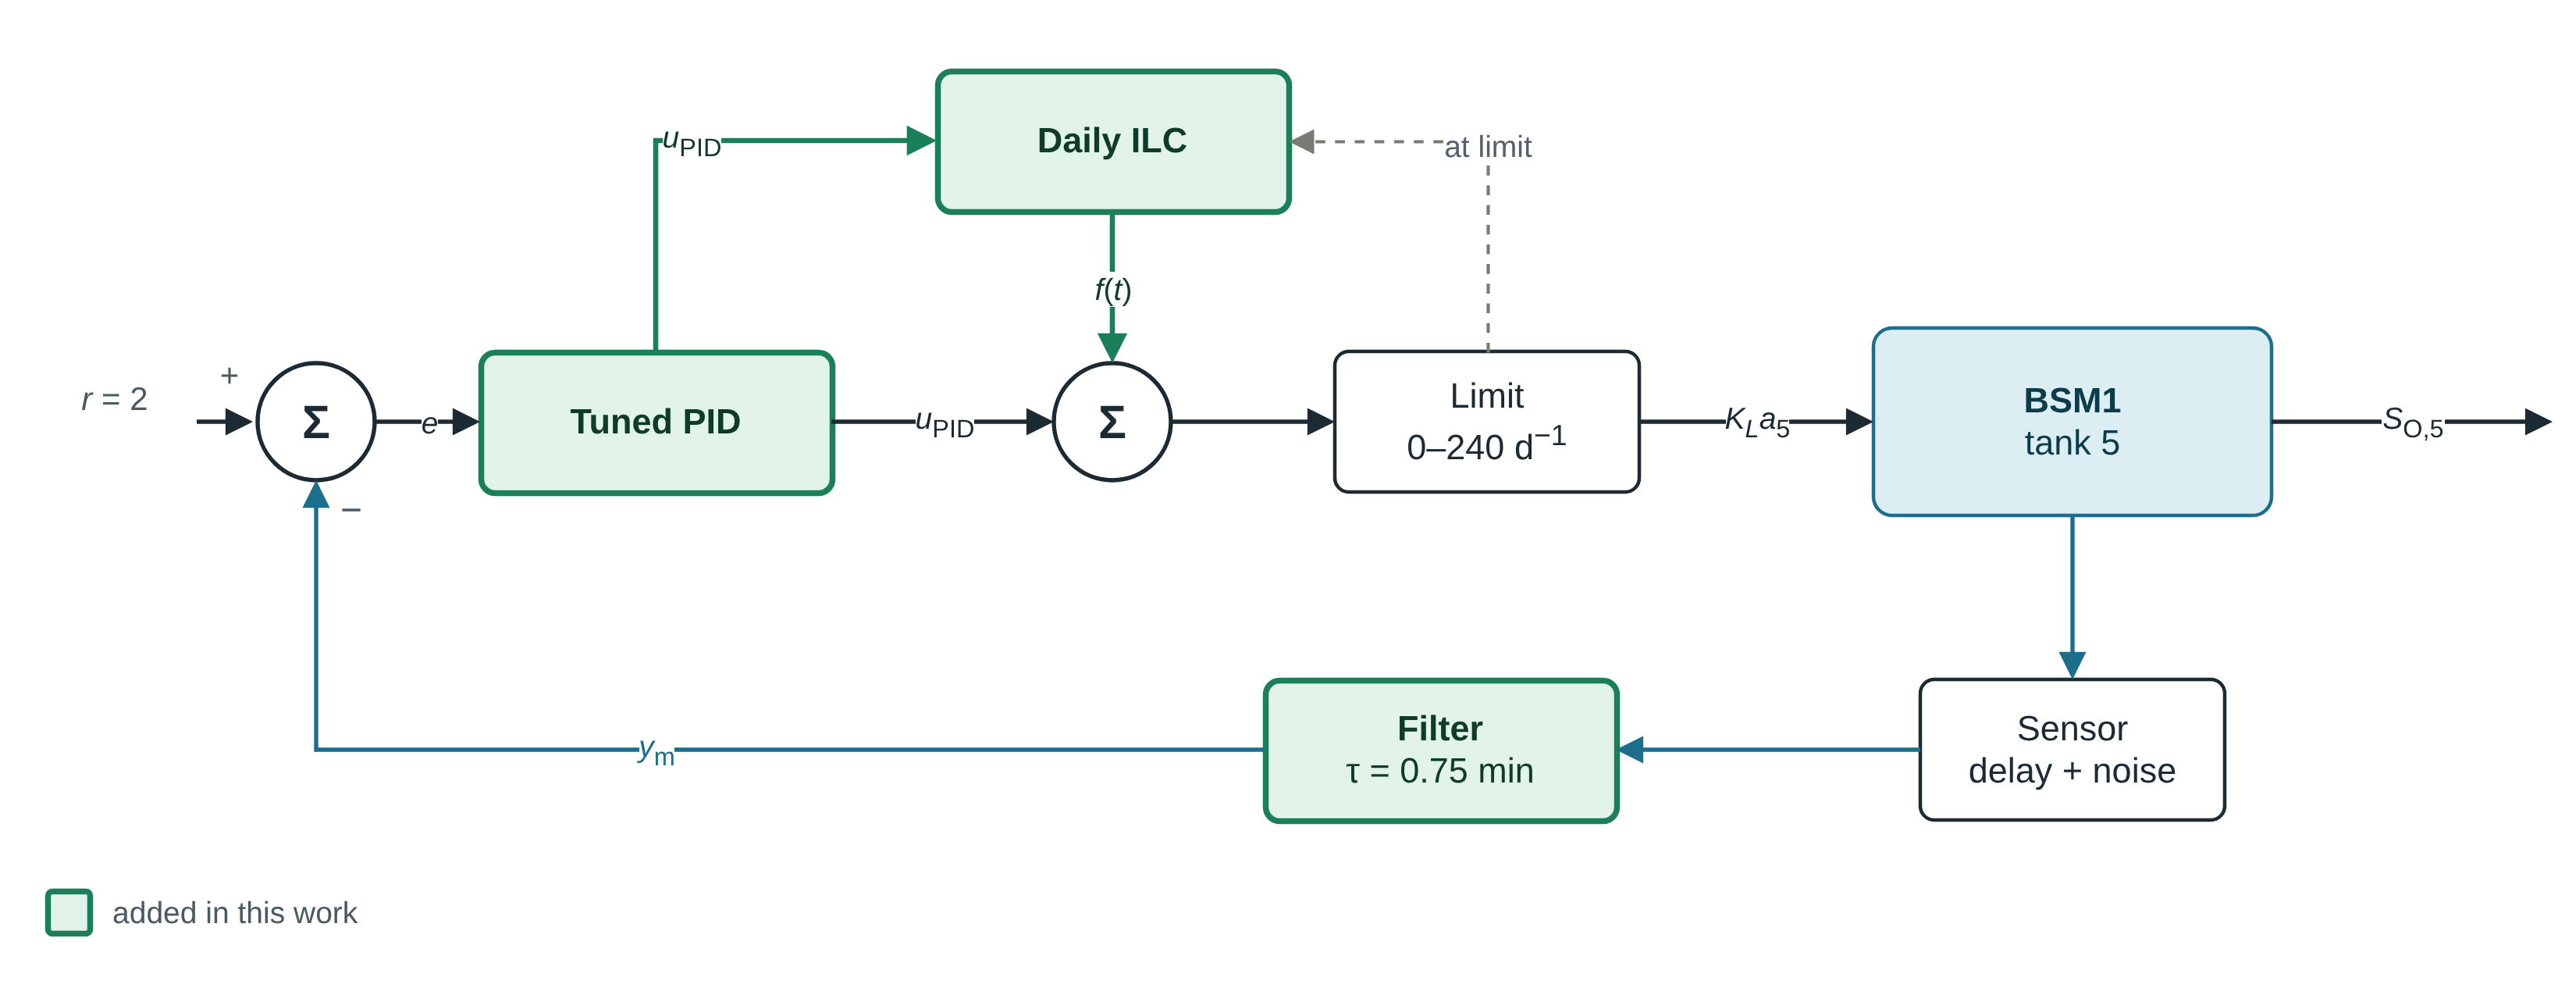
\includegraphics[width=0.86\textwidth]{d2_ours}
\caption{Architecture of our oxygen loop (robust variant). Green blocks are
added in this work: the PID with gains tuned per term, the daily ILC that
adds a feedforward $f(t)$, and a first-order filter on the measured oxygen.
The dashed arrow is the anti-windup signal: in slots where the aeration is
at a limit, the PID's limits are shifted by $f$ and the ILC does not learn.
The nitrate loop is the PID alone. A learned correction (SAC-IL or the
repaired MAACC, behind a safety gate) can be added at the second summing
junction; on the tuned PID with ILC it changes nothing, so it is not drawn.}
\label{fig:ours}
\end{figure*}
%=====================================================================

Table~\ref{tab:ctrl} lists the controllers compared. Everything that is
tuned or trained uses \emph{dry weather, days 0--7 only}.

\begin{table}[!t]
\centering
\caption{Controllers compared. Learned controllers have five training runs.}
\label{tab:ctrl}
\renewcommand{\arraystretch}{1.1}
\begin{tabular}{>{\raggedright\arraybackslash}p{0.33\columnwidth}>{\raggedright\arraybackslash}p{0.57\columnwidth}}
\toprule
Name & Description\\
\midrule
PID & paper's PID~\eqref{eq:pid}\\
MAACC & as printed in~\cite{wang2026maacc}\\
rMAACC & MAACC with repaired training, on the paper's PID\\
PID$\times$3 & all PID gains $\times3$\\
\quad +ILC & with the daily ILC on the oxygen loop\\
\quad +ILC+SAC-IL & with a gated SAC-IL correction\\
\quad +ILC+rMAACC & with a gated rMAACC correction\\
Tuned PID & P and I tuned per loop, D with P\\
\quad +ILC & with its own daily ILC\\
\quad +ILC-AW & with ILC anti-windup\\
\quad +ILC+SAC-IL & with a gated SAC-IL correction\\
Robust & tuned PID+ILC-AW, oxygen filter, gains $\times0.5$\\
\bottomrule
\end{tabular}
\end{table}

\subsection{Tuned PID}
The first baseline we built multiplies all of the paper's gains by one
factor. The loop becomes unstable at $\times5$; the largest whole factor
below 70\,\% of that is 3, giving PID$\times$3. This was too weak a baseline,
so we also tuned the P and I multipliers of each loop separately, each in
$\{1,2,3,4,6,8\}$ (36 settings per loop, D multiplier equal to P). A setting
is admissible only if it still finishes the training week with all its
multipliers raised by another factor of 1.5. The admissible setting with the
lowest training error is P$\times$2, I$\times$8, D$\times$2 for oxygen and
$\times3$ for nitrate. The oxygen choice sits at the edge of the grid, so a
larger search could find a still better PID.

\subsection{Daily iterative learning control}

\begin{figure}[!t]
\centering
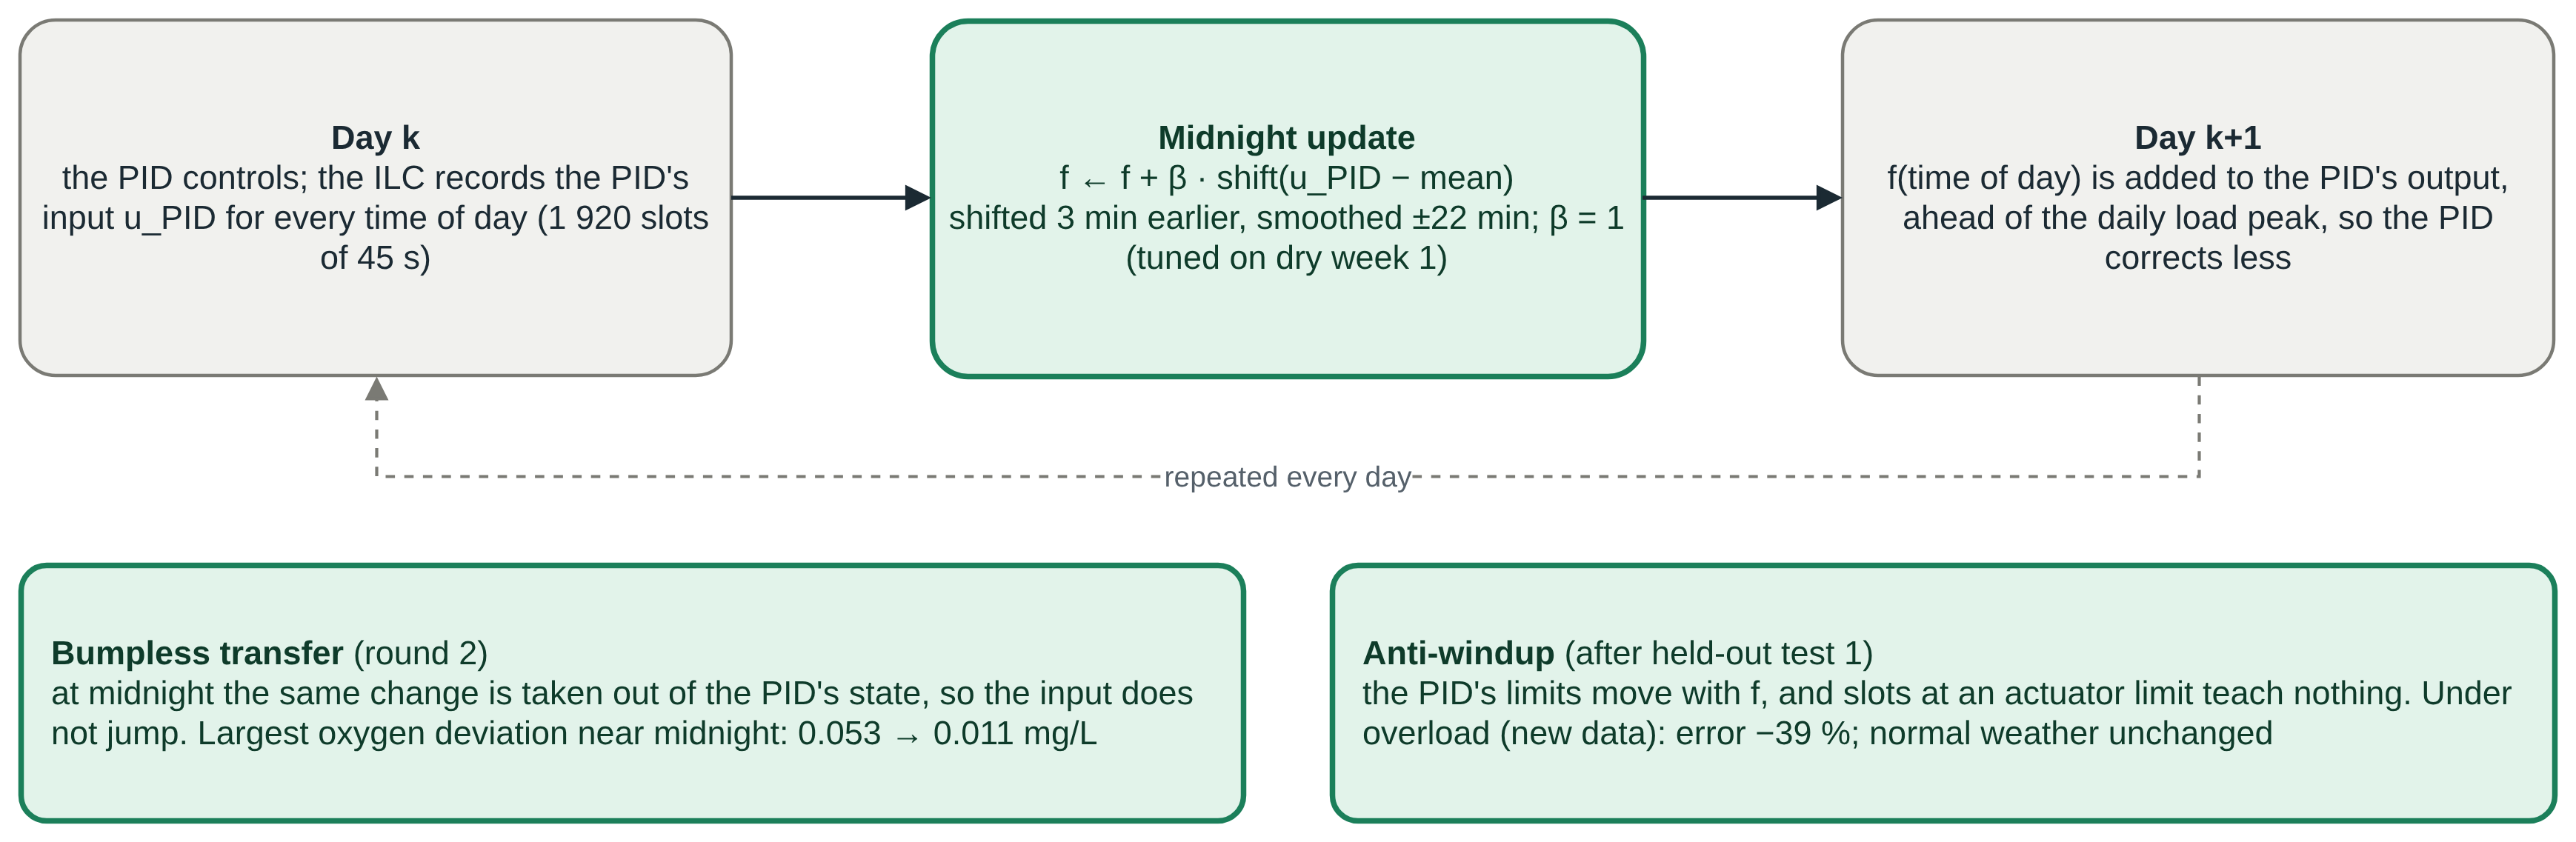
\includegraphics[width=\columnwidth]{d3_ilc}
\caption{The daily ILC, one update per night. $\mathcal{L}$ advances the
recorded profile by a few minutes and $\mathcal{S}$ smooths it, as in
\eqref{eq:ilc}. At the update the PID's state is reduced by the same
change, so the aeration does not jump at midnight.}
\label{fig:ilc}
\end{figure}

About 96\,\% of the oxygen error left by the PID repeats from one day to the
next: the PID reacts only after the daily load peak has moved the oxygen.
We therefore treat each day as one trial of a repeated task
(Fig.~\ref{fig:ilc}). With $j\in\{1,\dots,1920\}$ the 45-s slot of the day,
the aeration is
\begin{equation}
u_k = \mathrm{sat}\bigl(u^{\mathrm{PID}}_k + f_d(j_k)\bigr),
\end{equation}
and at the end of day $d$ the profile is updated as
\begin{equation}
f_{d+1} = \mathcal{S}_w\!\left[f_d + \beta\,\mathcal{L}_\ell\bigl(u^{\mathrm{PID}}_d-\overline{u^{\mathrm{PID}}_d}\bigr)\right],
\label{eq:ilc}
\end{equation}
where $\mathcal{L}_\ell$ advances the recorded profile by $\ell$ slots and
$\mathcal{S}_w$ is a circular moving average over $\pm w$ slots. The ILC
learns the correction the PID had to make and moves it into the feedforward,
as in feedback-error learning~\cite{gomi1993fel}. It starts from zero and
learns on-line.

Three details matter in practice.
\begin{itemize}
\item \emph{Bumpless update.} When the profile changes at midnight, the
  incremental PID's accumulated output is reduced by the same amount, so the
  total aeration does not jump. Before this change, all ten largest oxygen
  deviations of a dry run fell within 15 minutes of midnight; afterwards the
  largest deviation near midnight fell from 0.053 to 0.011\,mg/L.
\item \emph{Oxygen loop only.} A nitrate ILC tuned on dry days made nitrate
  worse in rain (test-week IAE 0.0146 against 0.0082 without it), so it
  was removed.
\item \emph{Anti-windup.} The PID's limits are shifted by the feedforward,
  to $[U_{\min}-f, U_{\max}-f]$, so the sum can reach either limit without
  the PID winding up. Slots spent at a limit are excluded from
  \eqref{eq:ilc}, and a day spent more than half at a limit keeps the old
  profile. This was added after held-out test~1 (Section~\ref{sec:h2}).
\end{itemize}
Algorithm~\ref{alg:ilc} gives the complete update.

\begin{algorithm}[!t]
\caption{Daily ILC with bumpless update and anti-windup}
\label{alg:ilc}
\begin{algorithmic}[1]
\Require share $\beta$, lead $\ell$, smoothing half-width $w$; $f(j)\gets0$ for all slots $j$
\For{each control step $k$, with $j$ its slot of the day}
  \State $u^{\mathrm{PID}}_k \gets$ PID step \eqref{eq:pid}, limited to $[U_{\min}-f(j),\,U_{\max}-f(j)]$
  \State apply $u_k \gets \mathrm{sat}(u^{\mathrm{PID}}_k+f(j))$
  \State record $g(j)\gets u^{\mathrm{PID}}_k$ and $o(j)\gets[u_k \text{ not at a limit}]$
  \If{$j$ is the last slot of the day}
    \If{$o$ is true in at least half of the slots}
      \State $\bar g \gets$ mean of $g$ over the slots with $o$ true
      \State $\delta(j)\gets o(j)\,\bigl(g(j)-\bar g\bigr)$ for all $j$
      \State $f^{+}\gets \mathcal{S}_w\bigl[f+\beta\,\mathcal{L}_\ell\,\delta\bigr]$
      \State PID state $\gets$ PID state $-\bigl(f^{+}(1)-f(1)\bigr)$ \Comment{bumpless}
      \State $f\gets f^{+}$
    \EndIf
  \EndIf
\EndFor
\end{algorithmic}
\end{algorithm}

The parameters were chosen on the training week by a rule fixed in advance:
the lowest oxygen IAE among settings whose largest oxygen deviation is no
larger than that of the PID alone. For PID$\times$3 this gives $\beta=0.75$,
$\ell=8$ slots (6\,min) and $w=30$; for the tuned PID, $\beta=1$, $\ell=4$
(3\,min) and $w=30$ ($\pm$22.5\,min). The error surface is flat around both
choices: for PID$\times$3, 24 of 60 settings are within 5\,\% of the best.

\subsection{SAC with imitation learning}


SAC-IL is our attempt to fix what we believe stops MAACC from learning: no
data re-use, a random start and no exploration. A small actor (18\,564
weights) sees the last three errors of both loops, both inputs and the
influent flow, and adds a bounded increment, at most 6\,d$^{-1}$ per period,
to the aeration at the second summing junction of Fig.~\ref{fig:ours}.
The reward is
$r=-(100|e_O|+50|e_N|)-0.05\|a\|^2$. Training on the dry training week
proceeds in four stages: a recorded run of the expert (PID with ILC),
behaviour cloning, a critic warm-up and five SAC~\cite{haarnoja2018sac}
episodes of seven days ($\gamma=0.97$, learning rate $3\times10^{-4}$, batch
256). The actor loss keeps an imitation term whose weight decays from 2 to
a floor of 0.5, as in TD3+BC~\cite{fujimoto2021td3bc}. A run takes about a
quarter of an hour on one CPU core, and the policy kept is the one with the
lowest oxygen and nitrate error on the training week. Only the aeration is
corrected; when SAC also moved the recycle, it traded nitrate for oxygen.

A \emph{safety gate} switches the learned part off for a step if any input
leaves its training range by more than 10\,\%, or if the expert's correction
exceeds what the learner is allowed to give.

\subsection{Repaired MAACC}
To separate MAACC's idea from its training, we kept its structure (one
agent per loop; each actor sees its own loop and outputs an increment; each
critic sees both loops and both actions; $u=a+b$) and replaced the training
with that of multiagent TD3~\cite{fujimoto2018td3,ackermann2019matd3}: a
replay buffer, target networks ($\tau=0.005$), twin critics, target-policy
smoothing (noise 0.2, clipped at 0.5), actor updates every second step, and
normalized inputs and reward. The actor's last layer is zero-initialized so
that the controller starts as its PID, and the increment is bounded by a
$\tanh$. It has neither the imitation term nor the entropy term of SAC-IL.
A first version that pre-trained on the expert's run alone, where the action
never varies, drifted before acting; it was replaced by the usual TD3
warm-up of one day of exploration. It has the same data and budget as
SAC-IL and was trained on the paper's PID (both loops) and, behind the same
gate, on PID$\times$3+ILC (oxygen only).

\begin{table}[!t]
\centering
\caption{Training settings of the two learned controllers. Both use dry
days 0--7 only, five episodes of seven days, and five training runs.}
\label{tab:train}
\renewcommand{\arraystretch}{1.08}
\begin{tabular}{lcc}
\toprule
 & SAC-IL & Repaired MAACC\\
\midrule
Discount $\gamma$ & 0.97 & 0.97\\
Learning rate & $3\times10^{-4}$ & $3\times10^{-4}$\\
Batch, replay buffer & 256, $4\times10^5$ & 256, $4\times10^5$\\
Target update $\tau$ & 0.005 & 0.005\\
Reward scale & 0.1 & 0.1\\
Increment bound per step & 6\,d$^{-1}$ ($K_La_{,5}$) & 6\,d$^{-1}$, 3000\,m$^3$/d\\
Start & behaviour cloning & last layer zero, 1-day warm-up\\
Exploration & entropy, $\alpha_0=0.005$ & Gaussian, std 0.1\\
Imitation term & weight $2\to0.5$ (floor) & none\\
Other & twin critics & twin critics, delay 2,\\
 & & target noise 0.2 (clip 0.5)\\
Loops corrected & oxygen & both (paper's PID)\\
\bottomrule
\end{tabular}
\end{table}

Table~\ref{tab:train} lists the training settings of both learners.

\subsection{Robust variant}
After held-out test~1 showed that every high-gain controller failed under
sensor noise, we searched, on the training week only and with the official
sensor models and two noise seeds (100, 101) that no test uses, for a
first-order filter on the measured oxygen and a scaling of the PID gains.
The chosen setting is a filter with $\tau=0.75$\,min and the tuned gains
halved in both loops, combined with the ILC with anti-windup. A first search
also filtered the nitrate measurement and made that loop oscillate; both
searches are kept in the repository.

%=====================================================================
\section{Evaluation Protocol}
%=====================================================================

\begin{figure}[!t]
\centering
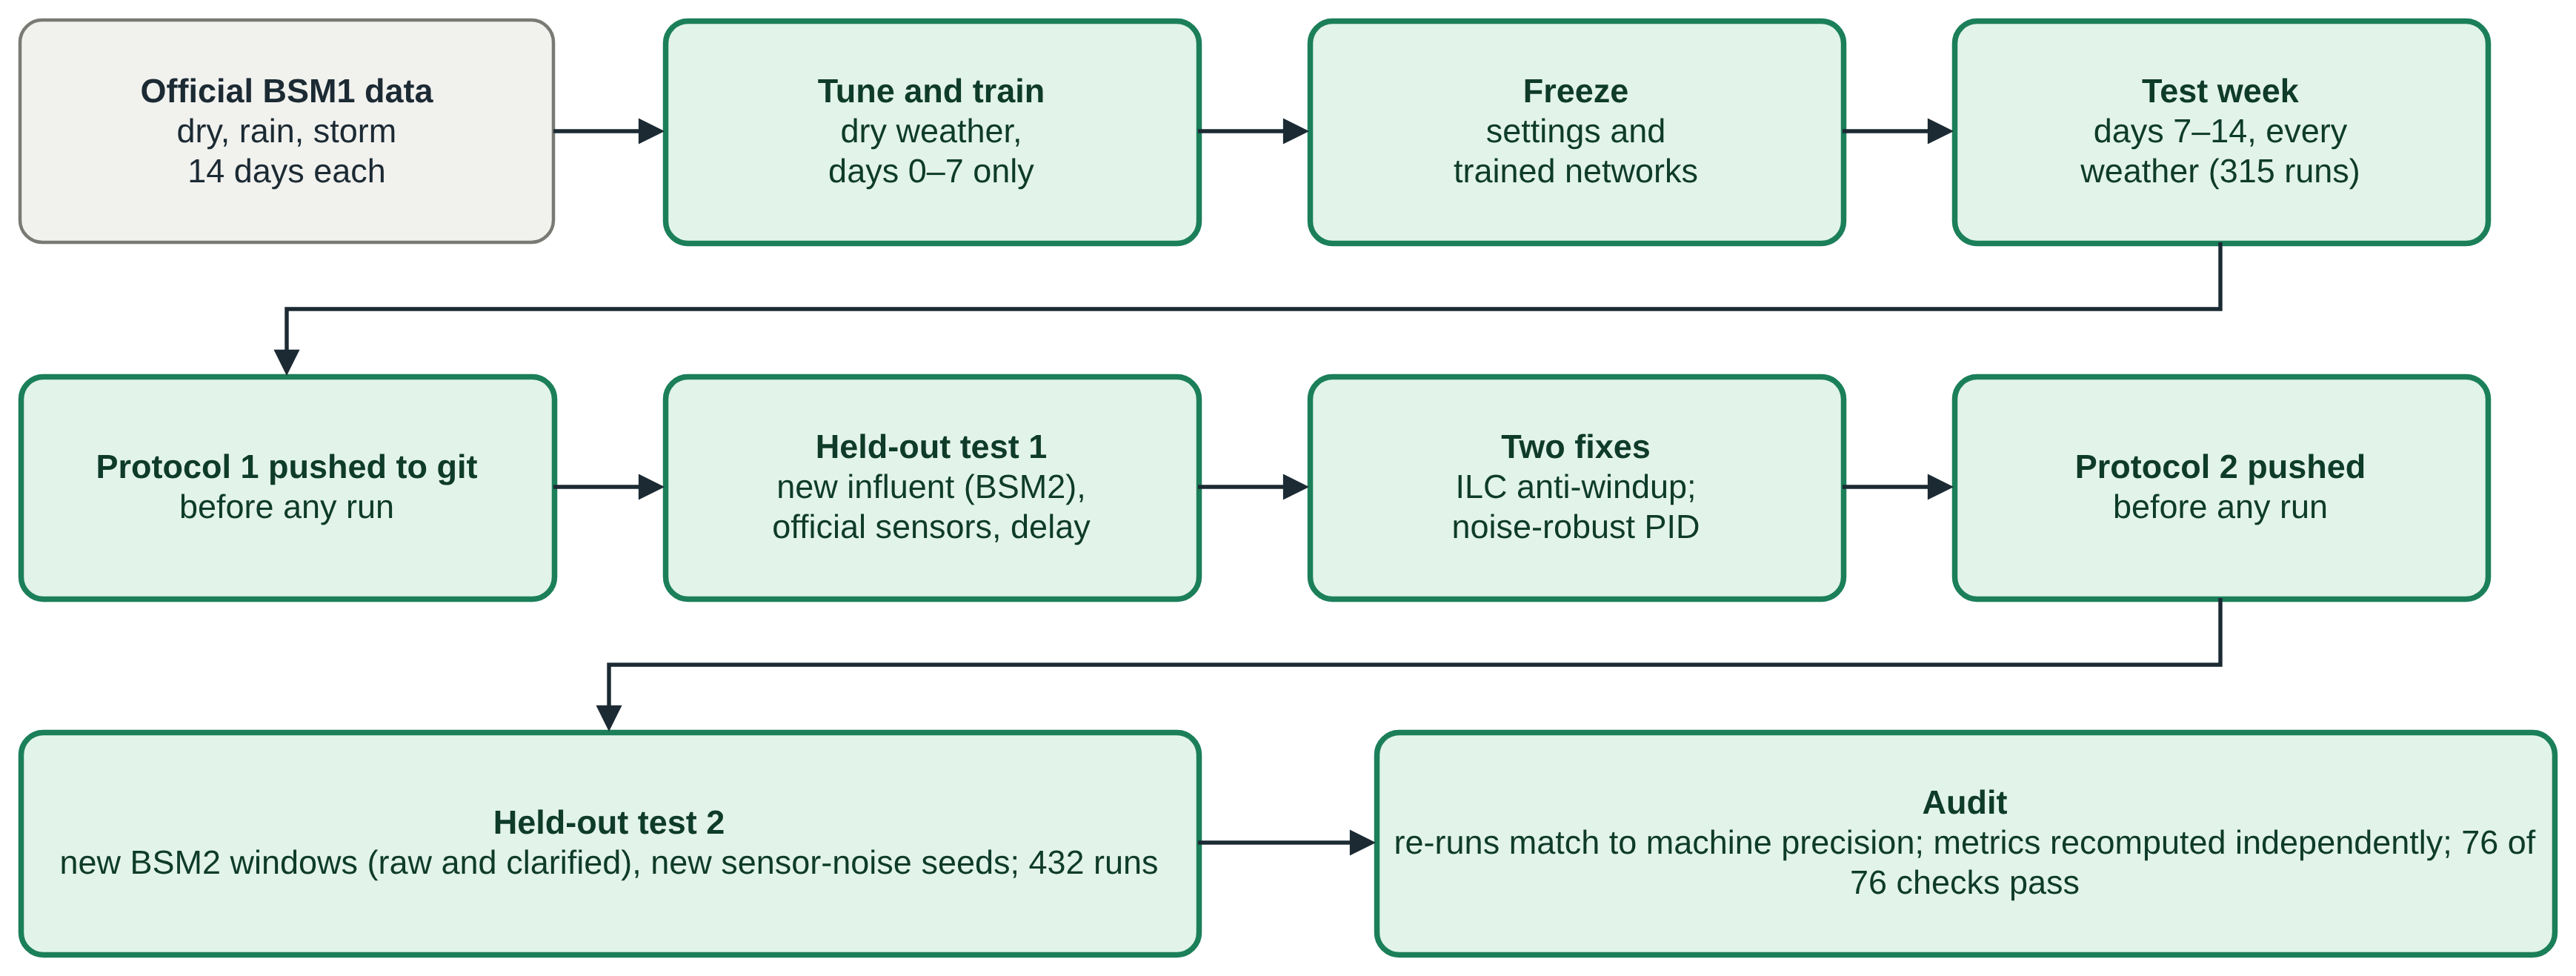
\includegraphics[width=\columnwidth]{d5_method}
\caption{Order of work. Each held-out protocol and the frozen controller
settings were committed and pushed before the first run of that test.}
\label{fig:method}
\end{figure}

Fig.~\ref{fig:method} gives the order in which the work was done.

\emph{Test week.} Each run lasts 14 days; tuning and training use only dry
days 0--7, and days 7--14 of every weather are the test (315 runs). The test
week contains the rain and storm events, so two of the three test
conditions were never seen in training. We also run 14 days of dry weather
with the paper's actuator noise (standard deviation 3\,\% of each upper
bound).

\emph{Held-out test 1}, protocol committed before any run:
\begin{itemize}
\item H1: six 14-day windows of the BSM2 influent~\cite{jeppsson2007bsm2},
  starting on days 245, 301, 357, 413, 469 and 525, with the flow scaled by
  0.878 to the BSM1 dry mean and temperature 15\,$^\circ$C;
\item H2: the official dry, rain and storm files with the official BSM1
  sensor models~\cite{alex2008bsm1}: oxygen class~A, $T_{90}=1$\,min;
  nitrate class~B$_0$, $T_{90}=10$\,min; white noise of standard deviation
  0.25\,mg/L on both; three noise seeds;
\item H3: as H2 with the sensor delays but no noise.
\end{itemize}
One amendment, adding SAC-IL on the tuned PID, was committed after the
test-week results and before any held-out run.

\emph{Held-out test 2}, committed after the two fixes and before any run:
\begin{itemize}
\item H4: six new BSM2 windows (days 273--553, no overlap with H1) with the
  particulate components halved, a fixed stand-in for a primary clarifier;
\item H5: the same windows without it, which overloads the plant;
\item H6: the official files with the official sensors and new seeds;
\item H7: H4 with the official sensors.
\end{itemize}
Held-out test 2 has 432 runs. Every held-out run starts from the same
state, lasts 14 days and is scored on days 7--14.

\emph{Comparisons.} A percentage compares a controller with the paper's PID
on only the windows or noise runs that both finished, so a controller's few
surviving runs are never compared with the PID's full set. We call one
controller \emph{better} than another only if its mean oxygen IAE is lower
\emph{and} it is better in at least two thirds of the windows or runs. This
rule was fixed in the protocols.

%=====================================================================
\section{Results}
%=====================================================================

\begin{figure*}[!t]
\centering
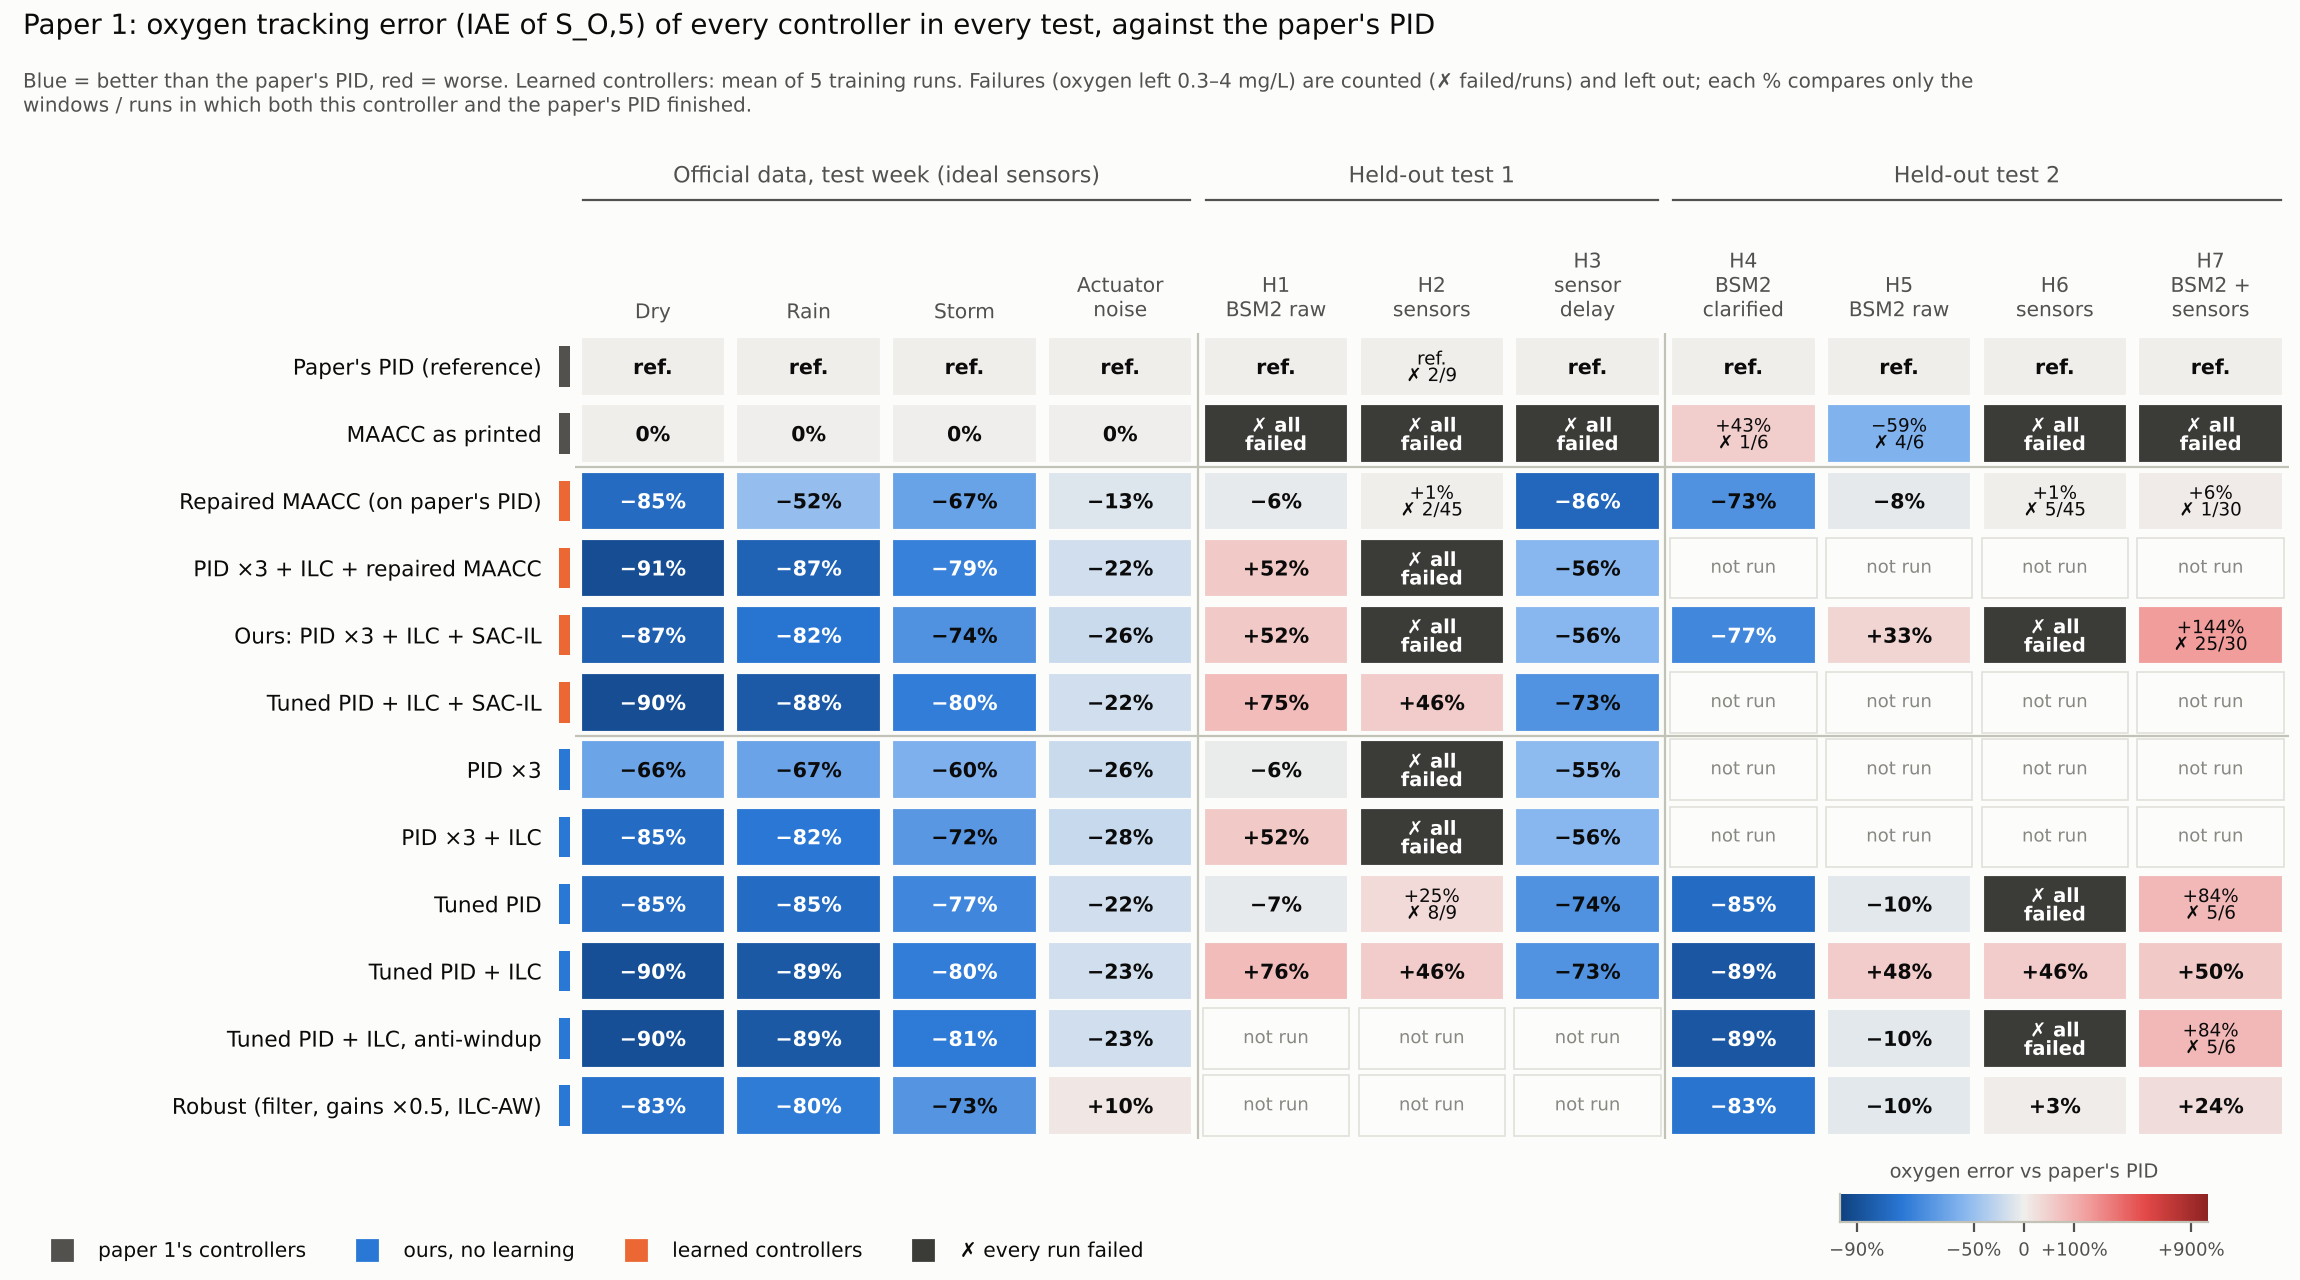
\includegraphics[width=0.9\textwidth]{f1_overview_matrix}
\caption{Every controller (row) in every test (column): change in oxygen IAE
against the paper's PID, paired over the runs both finished. Blue is better,
red worse; dark cells mean every run failed.}
\label{fig:matrix}
\end{figure*}

\begin{figure}[!t]
\centering
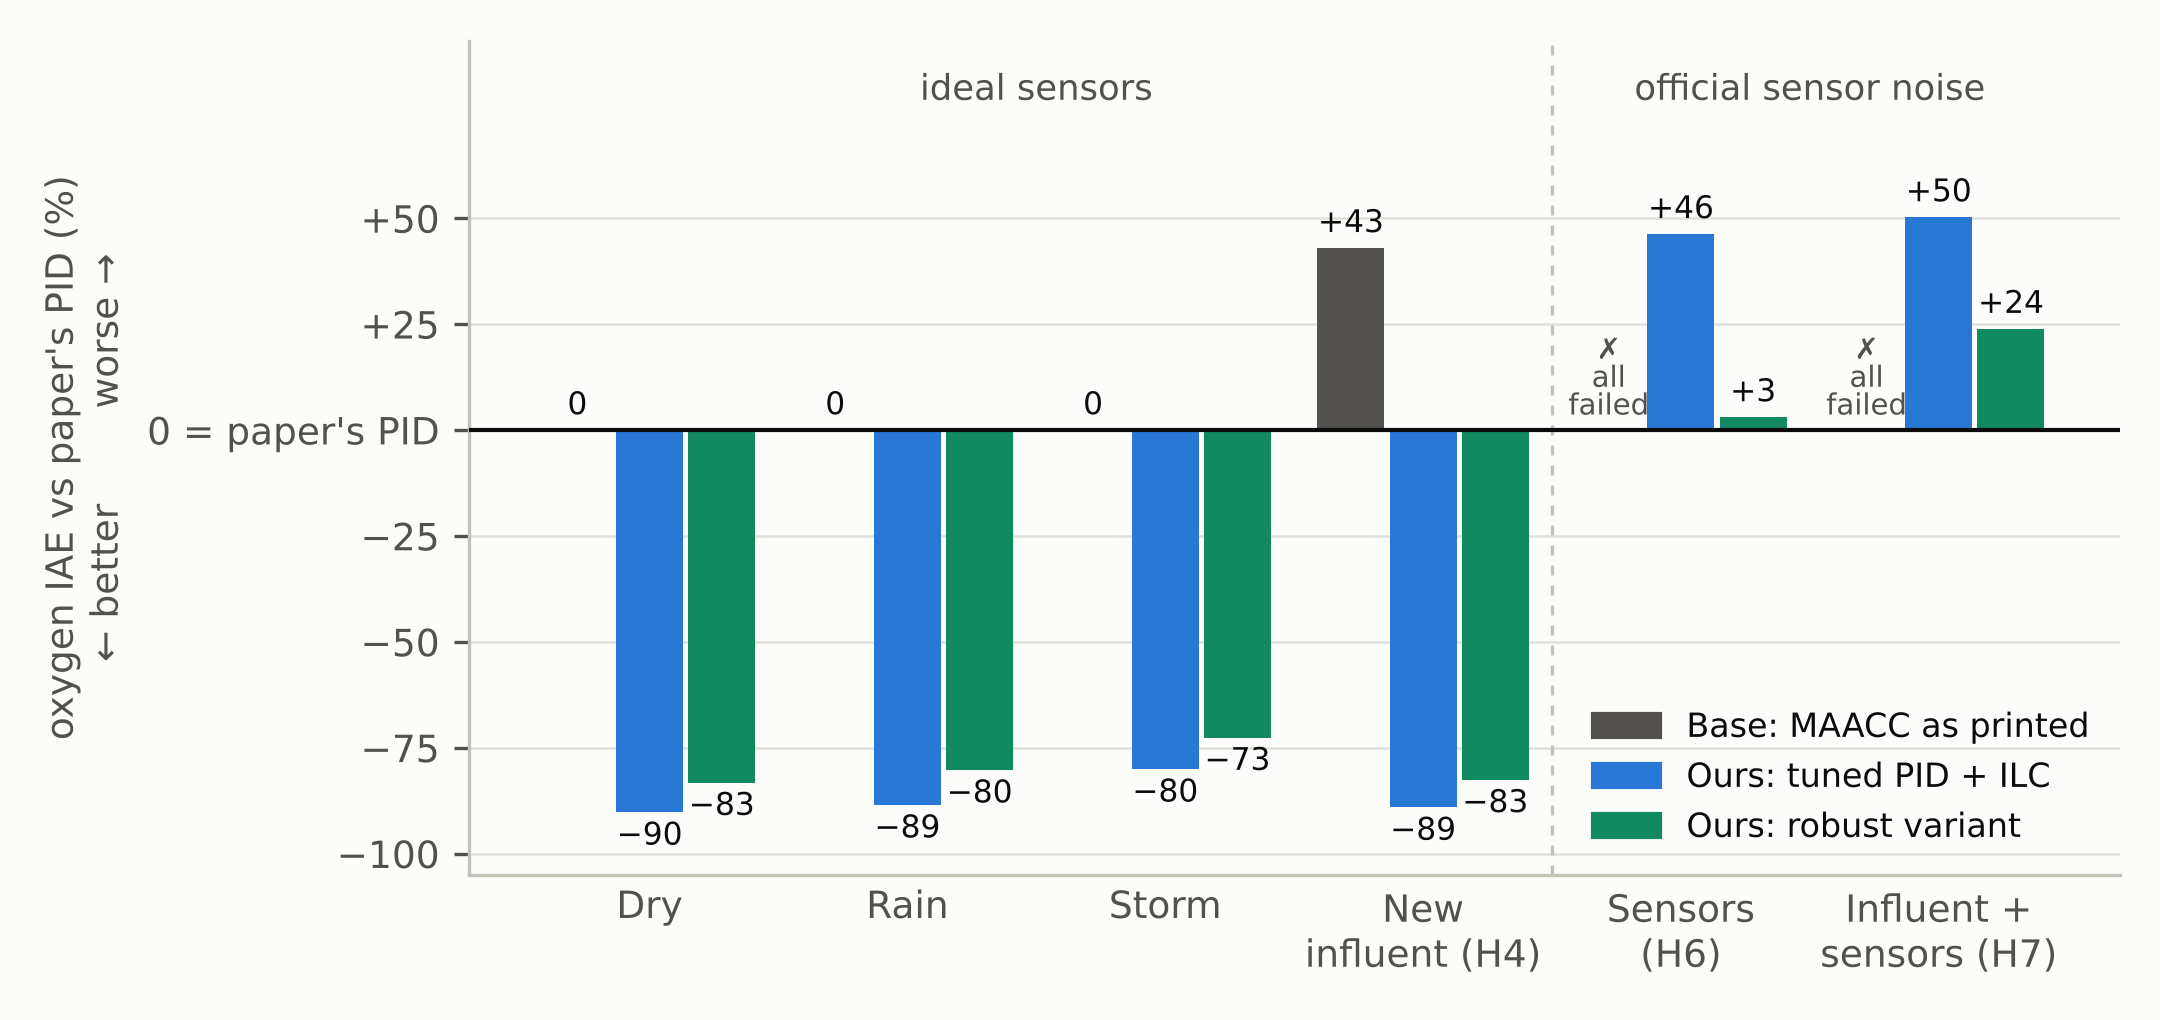
\includegraphics[width=\columnwidth]{f0_headline}
\caption{Base against ours, in brief: change in oxygen IAE against the
paper's PID (paired over the runs both finished). Left: ideal sensors, as in
the paper's own test, and new influent. Right: the official BSM1 sensor
noise. MAACC as printed lost 1 of 6 windows on new influent (H4).}
\label{fig:headline}
\end{figure}

Fig.~\ref{fig:headline} gives the main result in brief and
Fig.~\ref{fig:matrix} gives every controller in every test. The tables
below give the numbers.

\subsection{Test week}

\begin{table*}[!t]
\centering
\caption{Test week (days 7--14), oxygen IAE: change against the paper's PID
(first row: absolute IAE). Actuator noise: dry, 14 days. Movement: $K_La_{,5}$
movement per day, dry. Learned controllers: mean of five training runs.}
\label{tab:testweek}
\begin{tabular}{lccccc}
\toprule
Controller & Dry & Rain & Storm & Actuator noise & Movement (d$^{-1}$/day)\\
\midrule
PID (absolute IAE) & 0.0113 & 0.0100 & 0.0120 & 0.0249 & 501\\
MAACC as printed & \pc{0} & \pc{0} & \pc{0} & \pc{0} & 501\\
rMAACC & \pc{-85} & \pc{-52} & \pc{-67} & \pc{-13} & 1835\\
\midrule
PID$\times$3 & \pc{-66} & \pc{-67} & \pc{-60} & \pc{-26} & 966\\
PID$\times$3+ILC & \pc{-85} & \pc{-82} & \pc{-72} & \pc{-28} & 961\\
PID$\times$3+ILC+SAC-IL & \pc{-87} & \pc{-82} & \pc{-74} & \pc{-26} & 982\\
PID$\times$3+ILC+rMAACC & \pc{-91} & \pc{-87} & \pc{-79} & \pc{-22} & 1489\\
\midrule
Tuned PID & \pc{-85} & \pc{-85} & \pc{-77} & \pc{-22} & 852\\
Tuned PID+ILC & \pc{-90} & \pc{-89} & \pc{-80} & \pc{-23} & 852\\
Tuned PID+ILC+SAC-IL & \pc{-90} & \pc{-88} & \pc{-80} & \pc{-22} & 874\\
Robust & \pc{-83} & \pc{-80} & \pc{-73} & \pc{+10} & 522\\
\bottomrule
\end{tabular}
\end{table*}

\begin{figure}[!t]
\centering
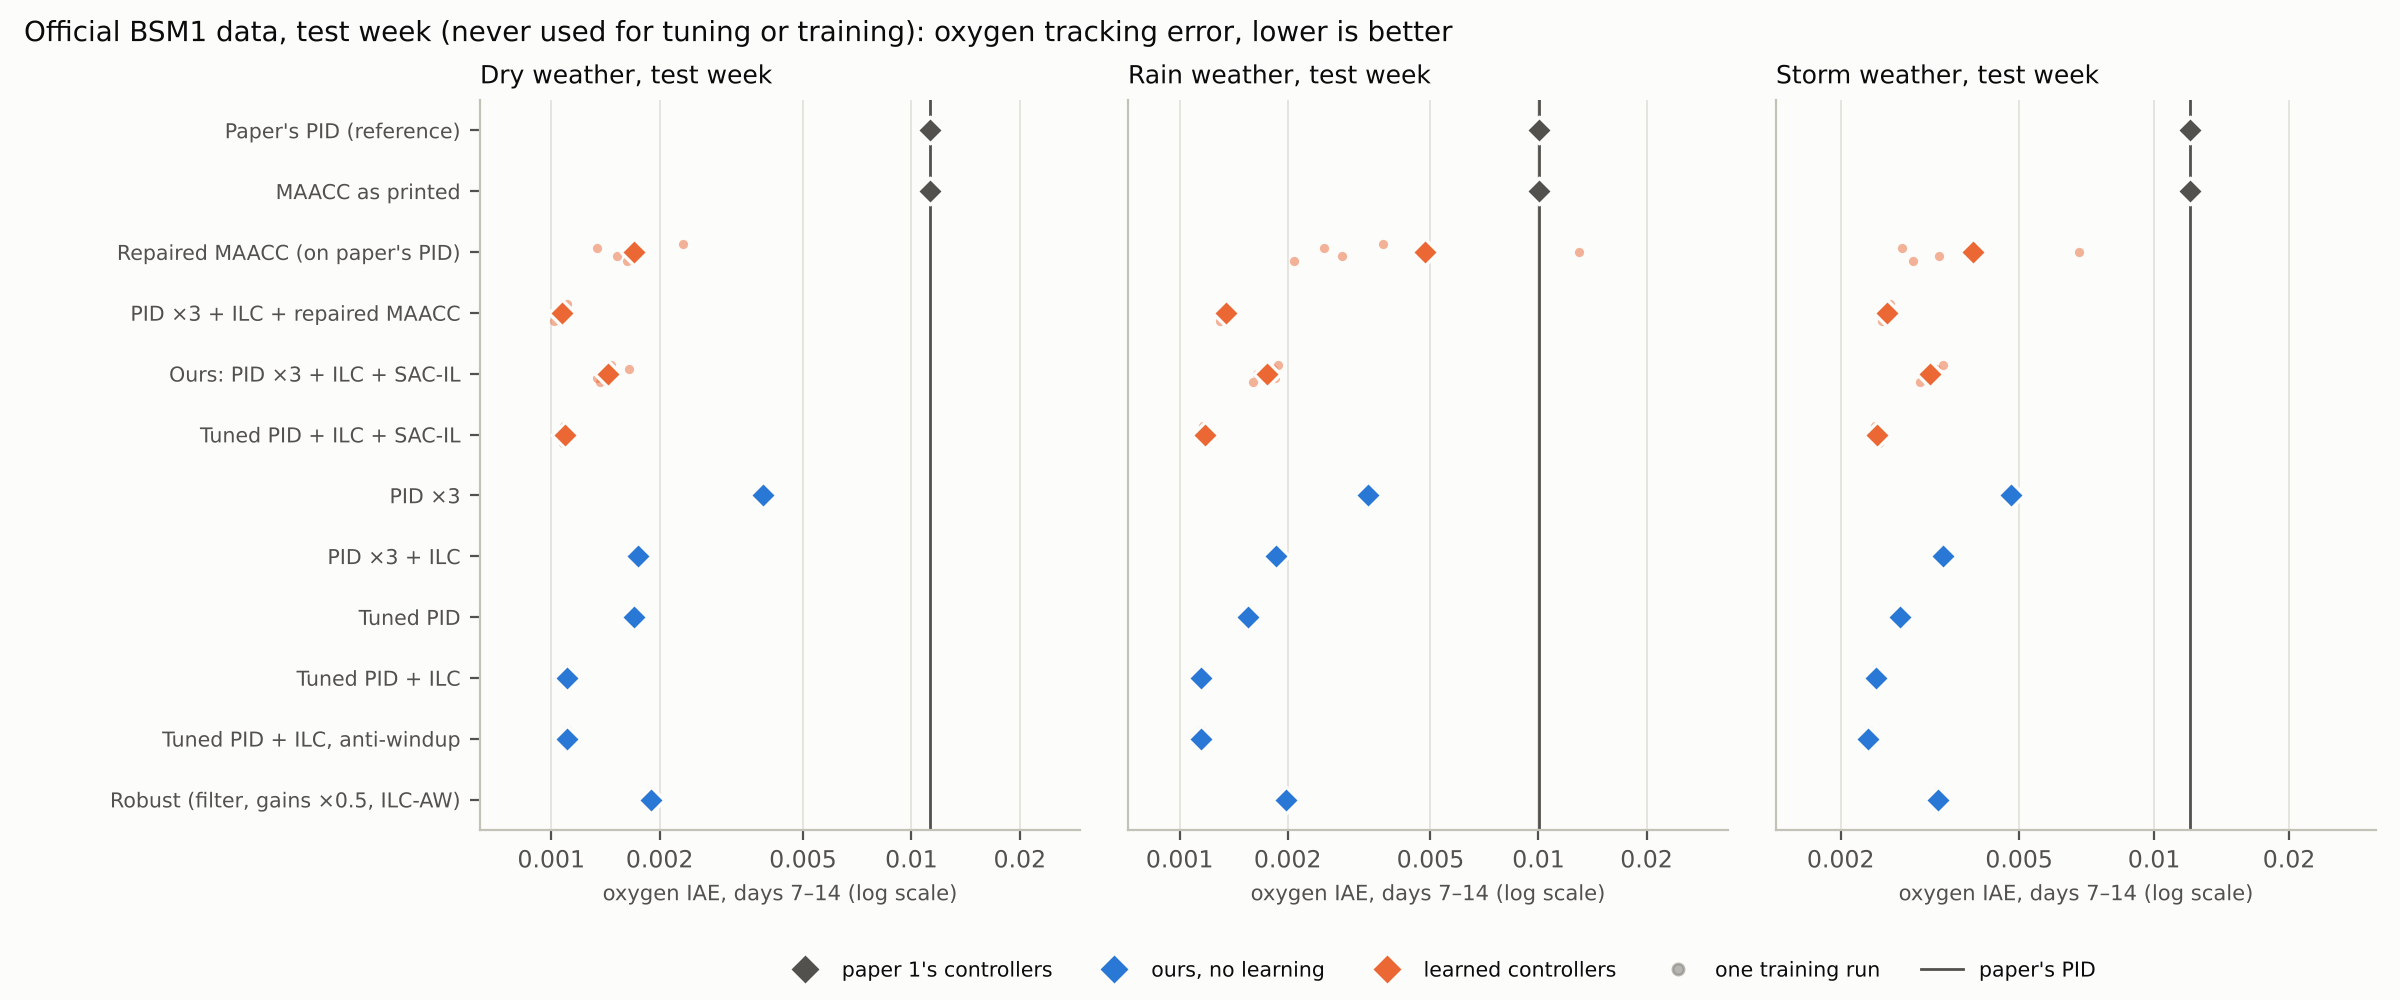
\includegraphics[width=\columnwidth]{f2_test_week}
\caption{Absolute oxygen IAE on the test week (log scale). Diamonds: means;
dots: the five training runs of a learned controller.}
\label{fig:testweek}
\end{figure}

Table~\ref{tab:testweek} and Fig.~\ref{fig:testweek} give the test-week
results. Four observations:
\begin{enumerate}
\item The paper's PID leaves a lot on the table. Tripling its gains alone
  removes 60--67\,\% of the oxygen error, and the tuned PID 77--85\,\%.
\item The ILC is the most useful single addition. It takes PID$\times$3
  from $-66$ to $-85$\,\% in dry weather and the tuned PID from $-85$ to
  $-90$\,\%.
\item SAC-IL adds 2 points on PID$\times$3+ILC in dry and storm weather, none
  in rain, and nothing on
  the tuned PID+ILC ($-90/-88/-80$\,\% with it, $-90/-89/-80$\,\% without).
  Without its gate, two of five trained policies extrapolate badly in rain
  and storm, and the mean oxygen error becomes 794 and 646\,\% larger than
  the PID's; the gate is on 0, 12.3 and 6.1\,\% of the time in dry,
  rain and storm, and 72.1\,\% with actuator noise.
\item Repaired, the paper's learner works. rMAACC reaches $-85$\,\% in dry
  weather, close to the paper's claim there, but only $-52$ and $-67$\,\%
  in rain and storm, and it moves the aeration 3.7 times as much as the
  PID. In the PID$\times$3+ILC stack it beats SAC-IL ($-91$ against
  $-87$\,\% dry) at 1.5 times the movement.
\end{enumerate}

\begin{figure}[!t]
\centering
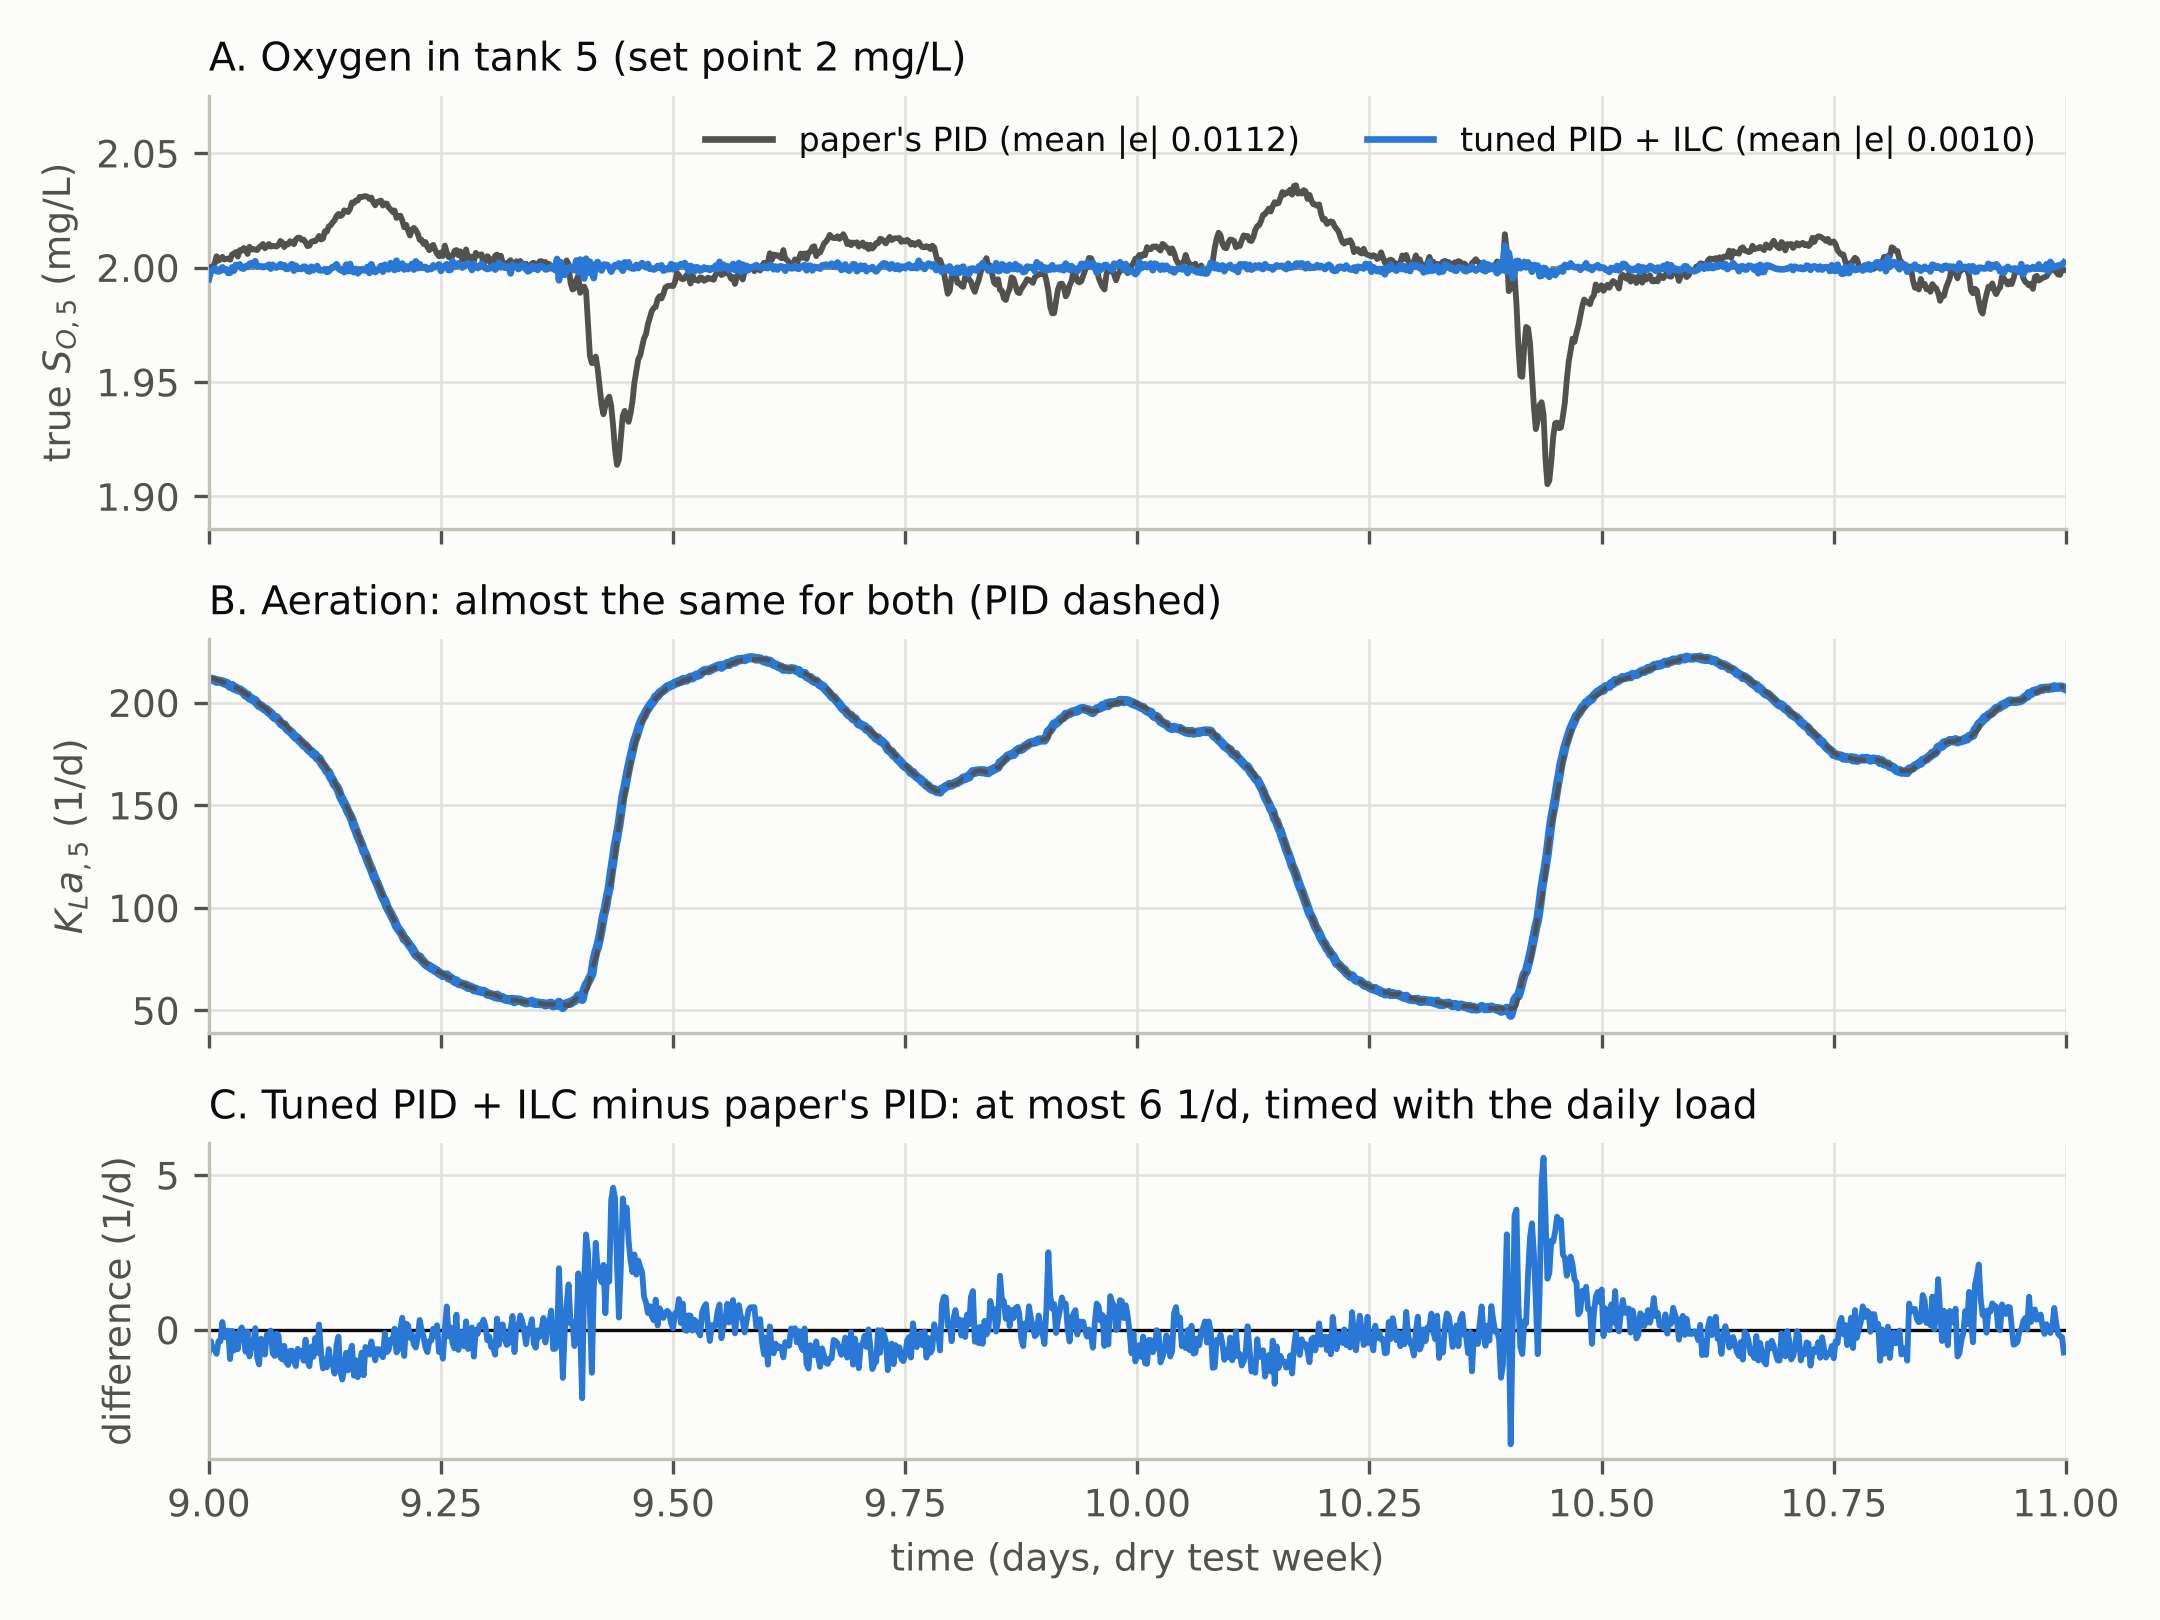
\includegraphics[width=\columnwidth]{f8_inside}
\caption{Two days of the dry test week. (a) True oxygen: the paper's PID
dips at every morning load rise; the tuned PID with ILC stays at the set
point (mean $|e|$ 0.0112 against 0.0010 over these two days). (b) The
aeration is almost the same for both. (c) The difference is at most
6\,d$^{-1}$, applied around the load rise: a small correction at the right
time is enough.}
\label{fig:inside}
\end{figure}

\begin{figure}[!t]
\centering
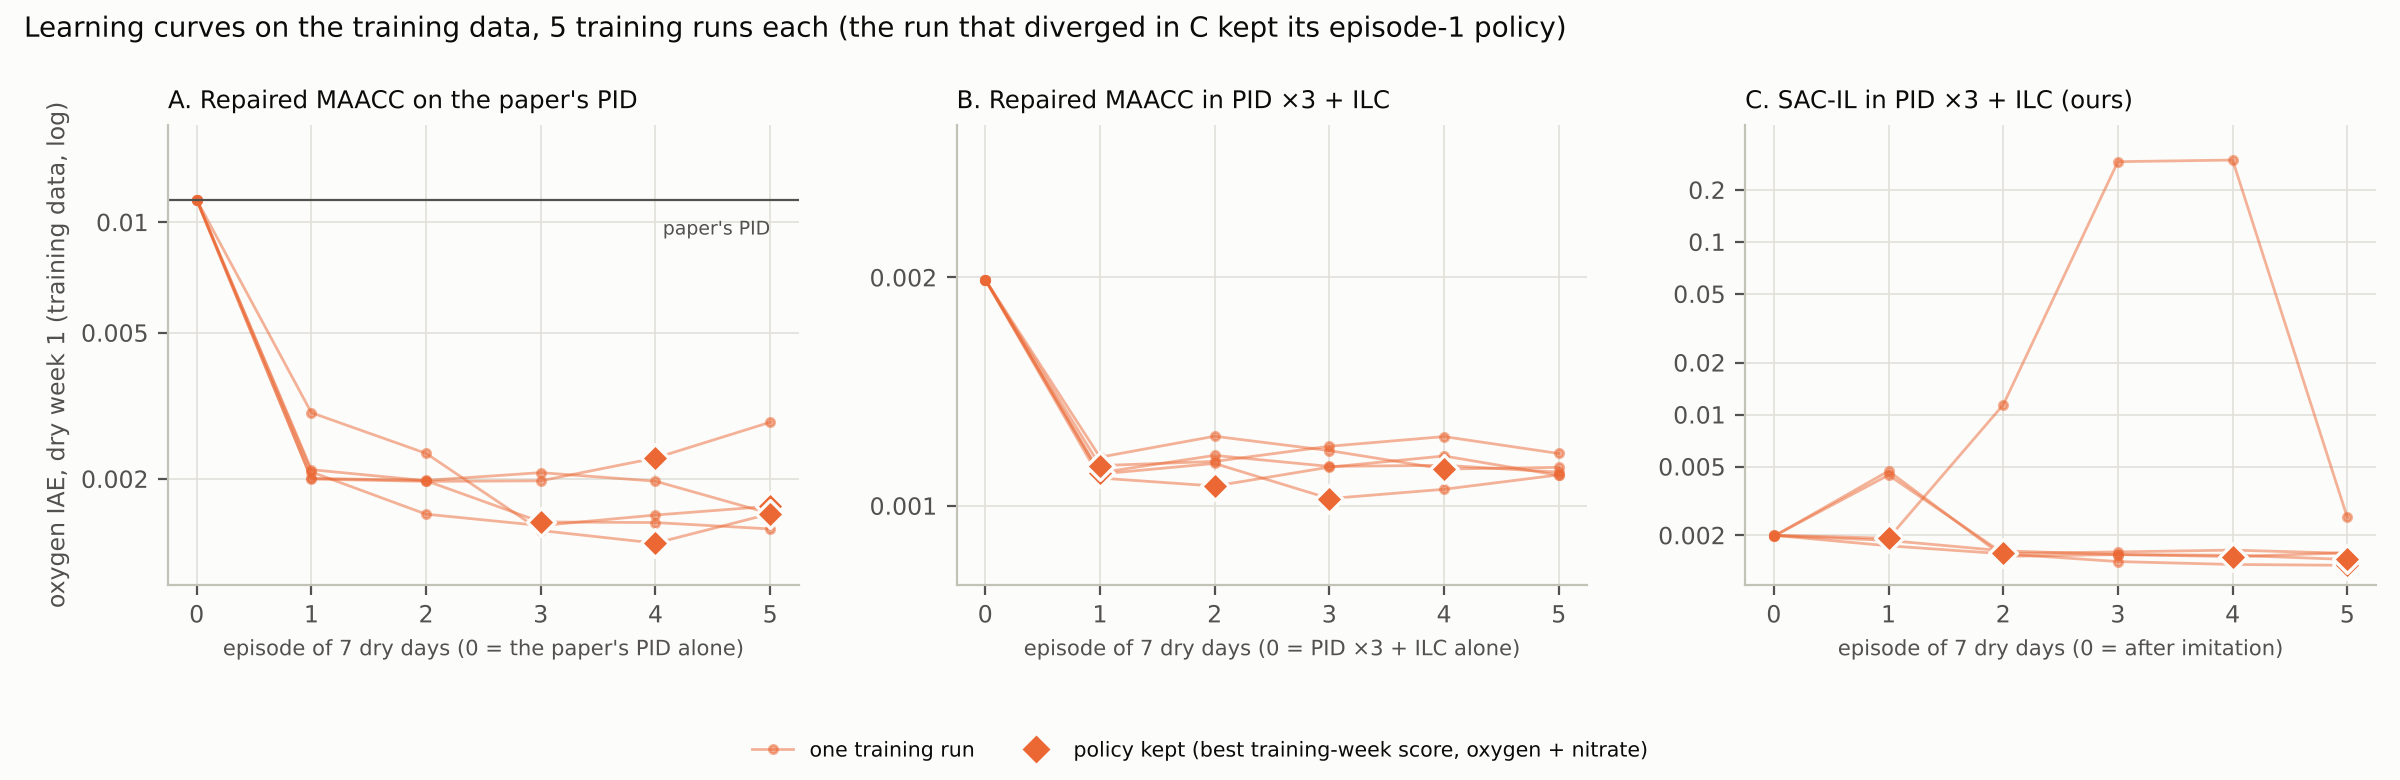
\includegraphics[width=\columnwidth]{f7_learning}
\caption{Oxygen IAE on the training week after each episode, five training
runs per learner. The repaired MAACC learns quickly from the paper's PID;
SAC-IL stays near its imitation start, and one run diverged.}
\label{fig:learning}
\end{figure}

Fig.~\ref{fig:inside} shows what the ILC does in the plant, and
Fig.~\ref{fig:learning} shows the learning curves. Aeration energy
(3690\,kWh/d in dry weather) and effluent ammonium (about 2.47\,g\,N/m$^3$)
are the same for all controllers to the precision reported. On nitrate, all
controllers built on PID$\times$3 or the tuned PID reach $-73/-46/-34$\,\%,
rMAACC $-62/-5/+6$\,\% and the robust variant $-36/-28/-15$\,\%.

\subsection{Held-out test 1}

\begin{table*}[!t]
\centering
\caption{Held-out tests, oxygen IAE on days 7--14: change against the
paper's PID over the runs both finished (first row: absolute IAE). F: every
run failed; (k/n): k of n runs failed; --: not run.}
\label{tab:heldout}
\setlength{\tabcolsep}{4.5pt}
\begin{tabular}{lccccccc}
\toprule
 & \multicolumn{3}{c}{Held-out test 1} & \multicolumn{4}{c}{Held-out test 2}\\
\cmidrule(lr){2-4}\cmidrule(lr){5-8}
Controller & H1 influent & H2 sensors & H3 delay & H4 influent & H5 overload & H6 sensors & H7 infl.+sens.\\
\midrule
PID (absolute IAE) & 0.106 & 0.255 (2/9) & 0.0319 & 0.0105 & 0.0815 & 0.261 & 0.178\\
MAACC as printed & \F & \F & \F & \pc{+43} (1/6) & \pc{-59} (4/6) & \F & \F\\
rMAACC & \pc{-6} & \pc{+1} (2/45) & \pc{-86} & \pc{-73} & \pc{-8} & \pc{+1} (5/45) & \pc{+6} (1/30)\\
\midrule
PID$\times$3 & \pc{-6} & \F & \pc{-55} & \na & \na & \na & \na\\
PID$\times$3+ILC & \pc{+52} & \F & \pc{-56} & \na & \na & \na & \na\\
PID$\times$3+ILC+rMAACC & \pc{+52} & \F & \pc{-56} & \na & \na & \na & \na\\
PID$\times$3+ILC+SAC-IL & \pc{+52} & \F & \pc{-56} & \pc{-77} & \pc{+33} & \F & \pc{+144} (25/30)\\
\midrule
Tuned PID & \pc{-7} & \pc{+25} (8/9) & \pc{-74} & \pc{-85} & \pc{-10} & \F & \pc{+84} (5/6)\\
Tuned PID+ILC & \pc{+76} & \pc{+46} & \pc{-73} & \pc{-89} & \pc{+48} & \pc{+46} & \pc{+50}\\
Tuned PID+ILC+SAC-IL & \pc{+75} & \pc{+46} & \pc{-73} & \na & \na & \na & \na\\
Tuned PID+ILC-AW & \na & \na & \na & \pc{-89} & \pc{-10} & \F & \pc{+84} (5/6)\\
Robust & \na & \na & \na & \pc{-83} & \pc{-10} & \pc{+3} & \pc{+24}\\
\bottomrule
\end{tabular}
\end{table*}

\begin{figure*}[!t]
\centering
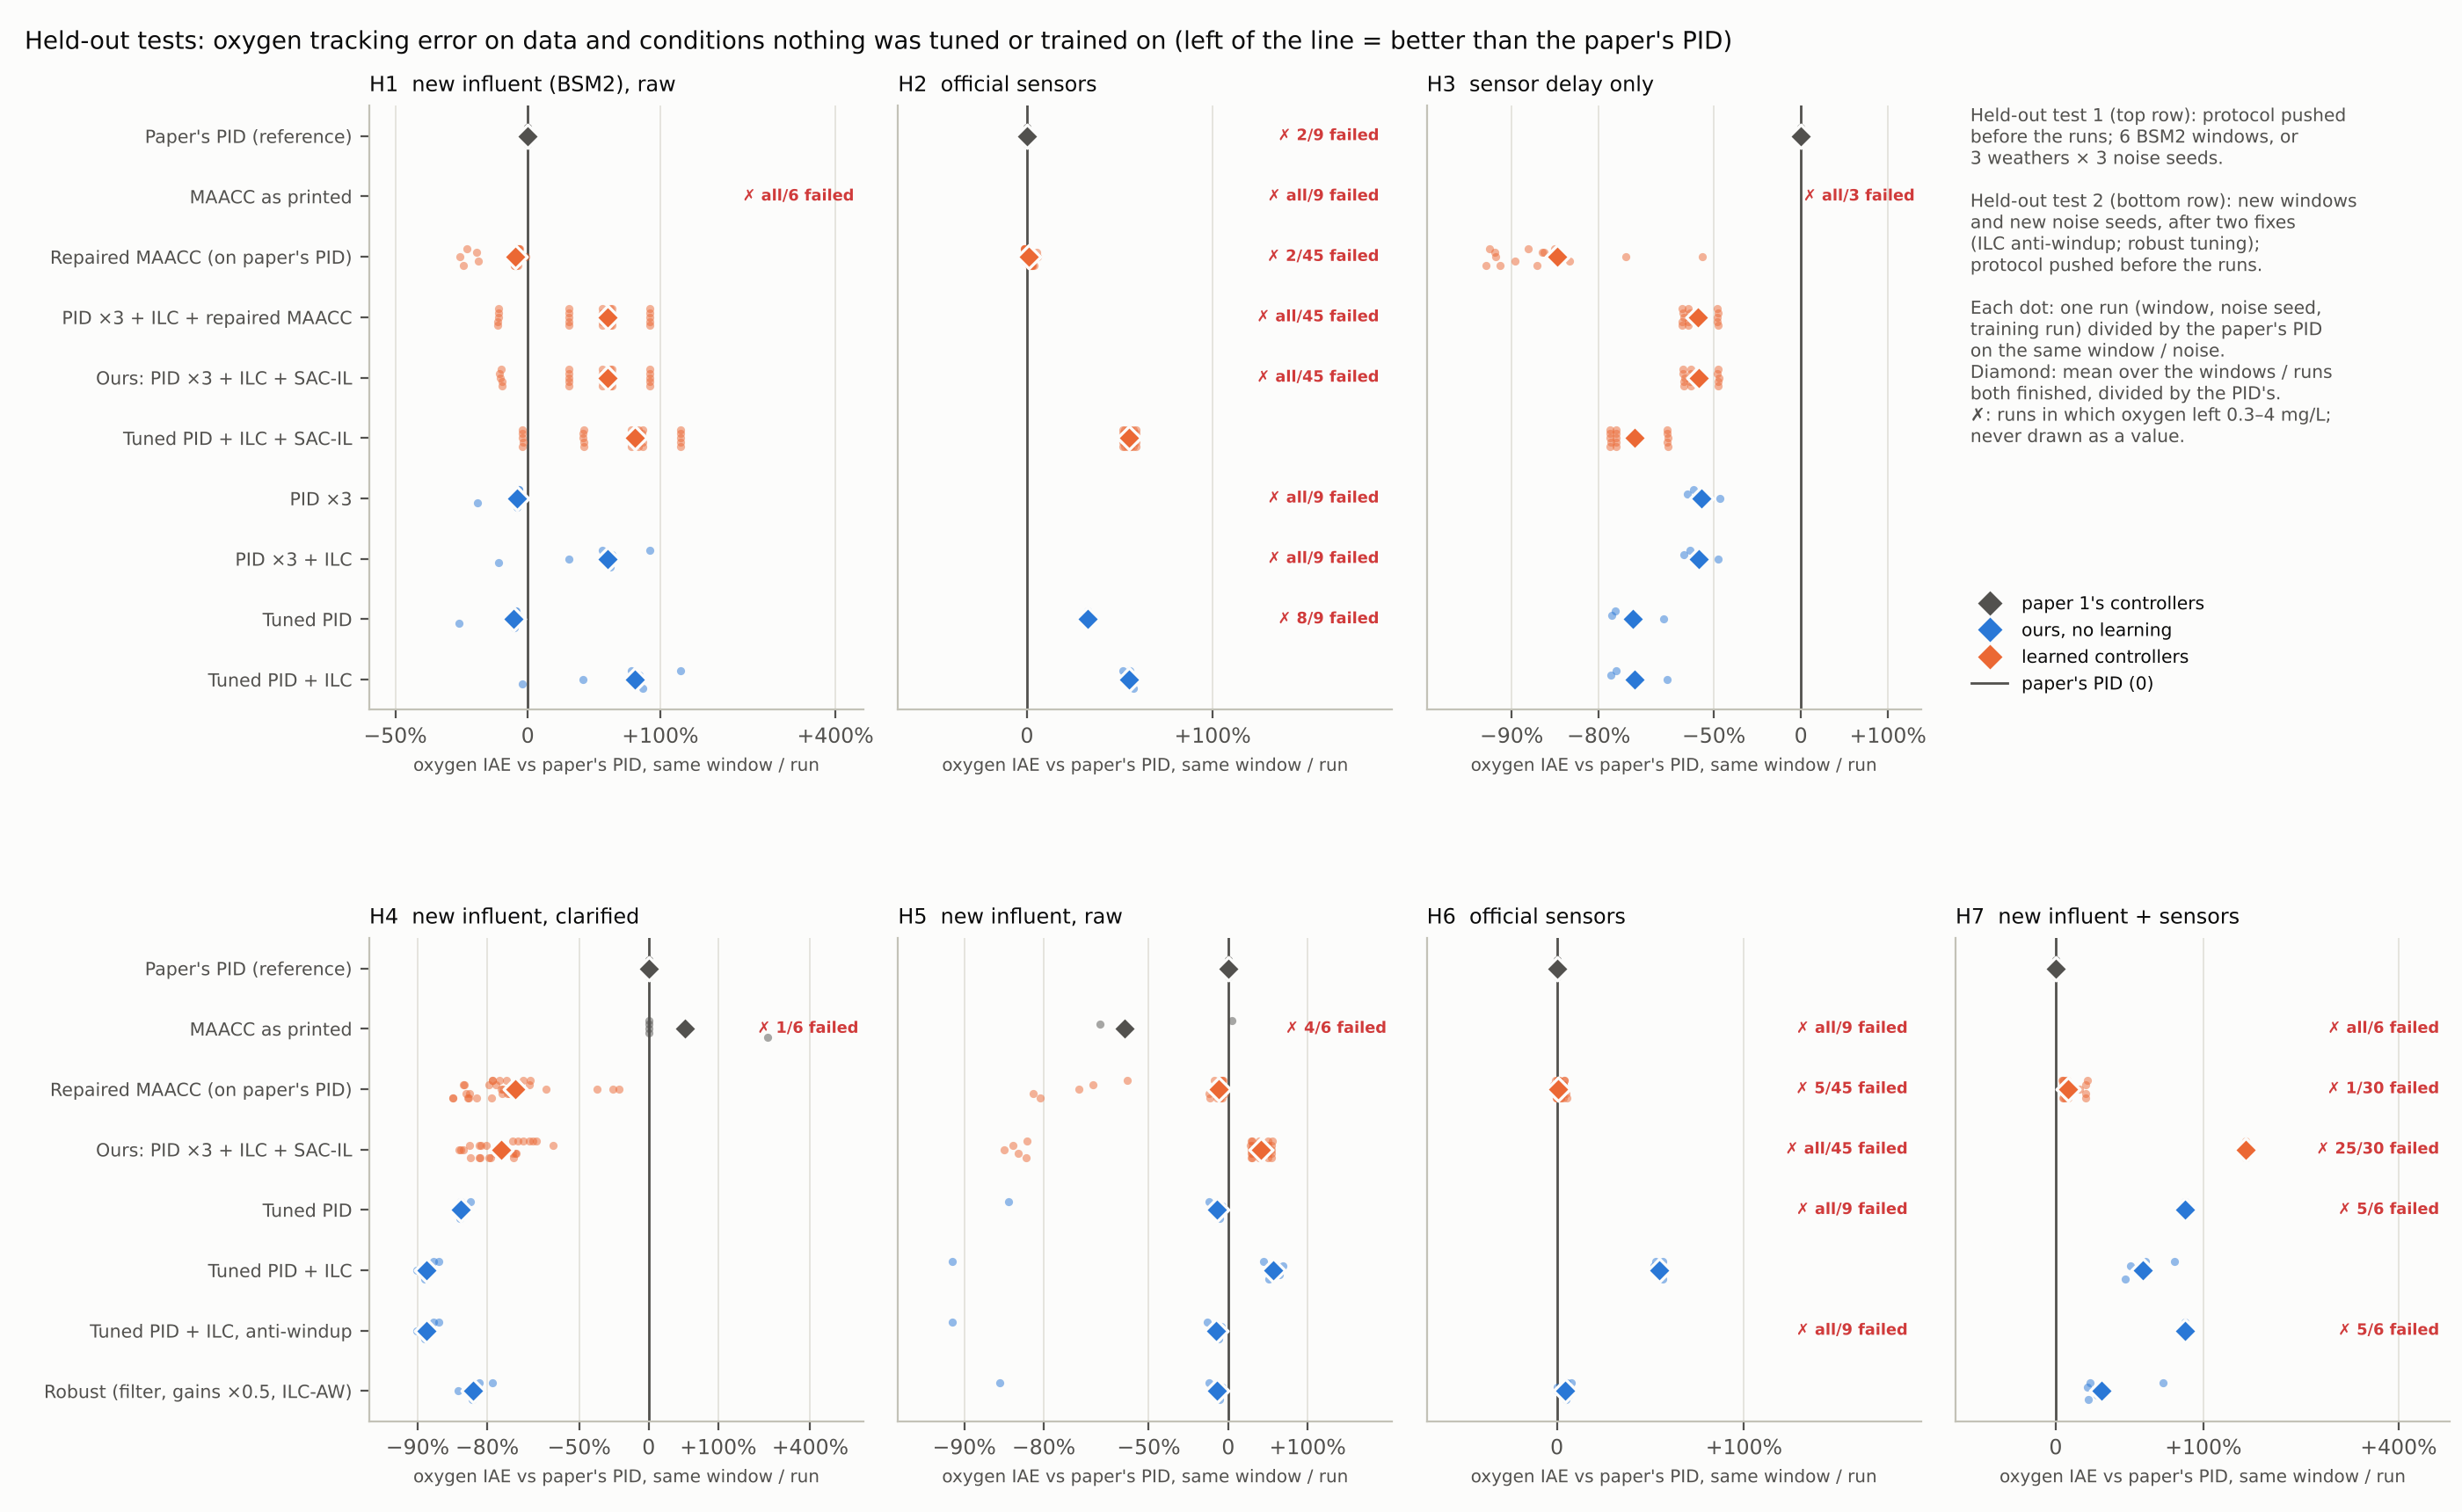
\includegraphics[width=0.9\textwidth]{f3_heldout}
\caption{Held-out tests. Each dot is one run (window, noise seed and
training run) divided by the paper's PID on the same window or noise. Left
of the line is better. Top: test~1; bottom: test~2.}
\label{fig:heldout}
\end{figure*}

Table~\ref{tab:heldout} and Fig.~\ref{fig:heldout} give the held-out
results. Test~1 did not go as we expected.

\emph{H1 overloaded the plant.} The BSM2 influent is raw sewage that in
BSM2 passes a primary clarifier first. Fed straight into BSM1, it keeps the
aeration at its upper limit about 30\,\% of the time, and every controller's
error is about ten times larger than in the test week. We had not foreseen
this when writing the protocol. Under saturation the ILC made things worse
($+52$\,\% on PID$\times$3, $+76$\,\% on the tuned PID): it learns a
feedforward the actuator cannot deliver and releases it when the saturation
ends.

\emph{H2: high gains do not survive sensor noise.} With the official sensor
noise, PID$\times$3 and everything built on it left the safe range within
half a day in every run, including our SAC-IL controller. The tuned PID
failed 8 of 9 runs. The paper's PID and rMAACC each lost the same noise seed
in dry and storm weather; the tuned PID+ILC finished every run with a 46\,\%
larger error than the paper's PID.

\emph{H3: with sensor delay alone,} rMAACC was the best controller
($-86$\,\%), ahead of the tuned PID ($-74$\,\%).

On H1--H3 the safety gate kept the learned corrections off 96--100\,\% of
the time, so they neither helped nor harmed: each gated controller equals its
base.

\subsection{Held-out test 2}
\label{sec:h2}

The two failures of test~1 led to the two fixes of Section~\ref{sec:ctrl}: ILC
anti-windup and the robust variant. Both were frozen and committed, with the
test-2 protocol and its five pre-declared questions, before any test-2 run.

\begin{figure}[!t]
\centering
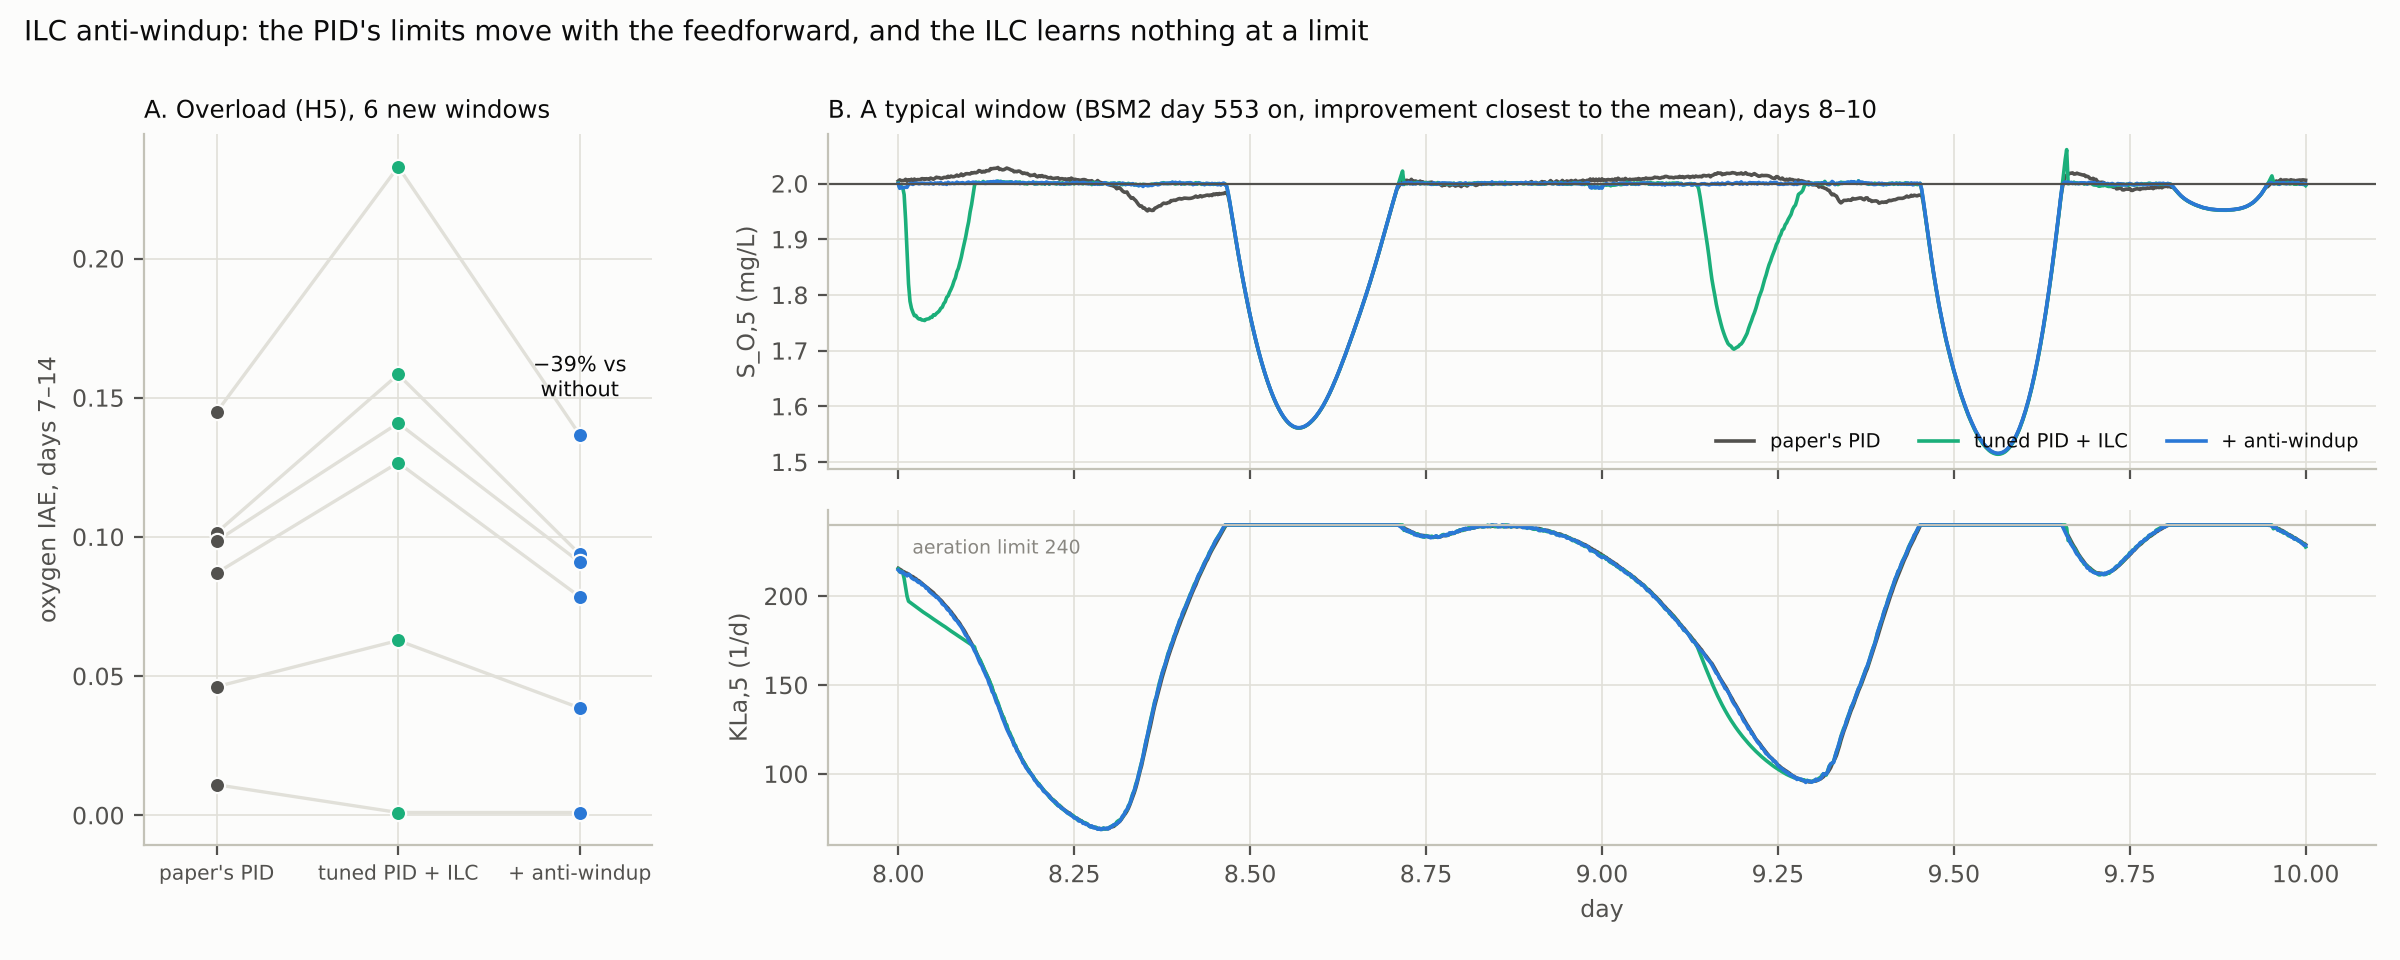
\includegraphics[width=\columnwidth]{f5_antiwindup}
\caption{ILC anti-windup under overload (H5). (a) Oxygen IAE in the six
windows. (b) The window whose improvement is closest to the mean: without
anti-windup the oxygen drops when the aeration leaves its limit.}
\label{fig:aw}
\end{figure}

\emph{Anti-windup works.} On H5, the ILC with anti-windup has a 39\,\%
lower error than without it and is better in 5 of 6 windows; on H4 the
difference is 0.0\,\% (Fig.~\ref{fig:aw}). With anti-windup the tuned
PID+ILC is no worse than the tuned PID under overload ($-10$\,\% against the
paper's PID for both). Anti-windup is not free, however. Under the official
sensor noise the tuned PID+ILC with anti-windup fails every H6 run and 5 of
6 H7 windows, as the tuned PID alone does, whereas without anti-windup it
finished every run. With noise the loop reaches its limits often, and
anti-windup lets the high-gain PID move straight from one limit to the
other. It needs lower gains, which is what the robust variant has.

\emph{The robust variant never fails, but it does not beat the paper's PID
under noise.} It finished all H6 and H7 runs, as did the paper's PID, and
was 3 and 24\,\% worse than the paper's PID there, better in none of the
runs. With ideal sensors it is better than the paper's PID in every window
of H4 ($-83$\,\%) and H5 ($-10$\,\%), and it keeps the paper's aeration
movement (522 against 501\,d$^{-1}$/day). The price of robustness on H4 is
a 60\,\% larger error than the tuned PID+ILC-AW (0.0018 against 0.00115).

\emph{rMAACC is the most consistent learned controller.} It is $-73$\,\% on
H4 and $-8$\,\% on H5, and close to the paper's PID with sensor noise ($+1$\,\%
on H6, $+6$\,\% on H7), with a few failed runs. By the pre-declared rule it
is not better than the paper's PID on H4--H7 as a whole.

\begin{table}[!t]
\centering
\caption{The questions declared in the protocol of held-out test~2, and
their answers. ``Better'' requires a lower mean and better in at least two
thirds of the windows or runs.}
\label{tab:questions}
\renewcommand{\arraystretch}{1.1}
\begin{tabular}{>{\raggedright\arraybackslash}p{0.42\columnwidth}>{\raggedright\arraybackslash}p{0.30\columnwidth}>{\raggedright\arraybackslash}p{0.16\columnwidth}}
\toprule
Question & Result & Answer\\
\midrule
(i) Anti-windup better than without it under overload (H5)? & $-39$\,\%, 5 of 6 windows & yes\\
\quad and no worse on normal influent (H4)? & 0.0\,\% & yes\\
(ii) Robust variant fails less than the paper's PID with sensors (H6, H7)? & neither failed & no difference\\
\quad and is it better there? & $+3$, $+24$\,\%; 0 runs better & no\\
(iii) Price of robustness on H4, against tuned PID+ILC-AW & $+60$\,\% & reported\\
(iv) Robust variant better than the paper's PID on H4 and H5? & $-83$, $-10$\,\%; 6 of 6 each & yes\\
(v) Repaired MAACC better than the paper's PID on H4--H7? & H4, H5: yes; H6, H7: no & no overall\\
\bottomrule
\end{tabular}
\end{table}

Table~\ref{tab:questions} answers the five questions declared in the
protocol of this test.

\emph{Our SAC-IL controller does not generalize.} It failed every H6 run and
25 of 30 H7 runs, and on H5 it was 33\,\% worse than the paper's PID.

\begin{figure}[!t]
\centering
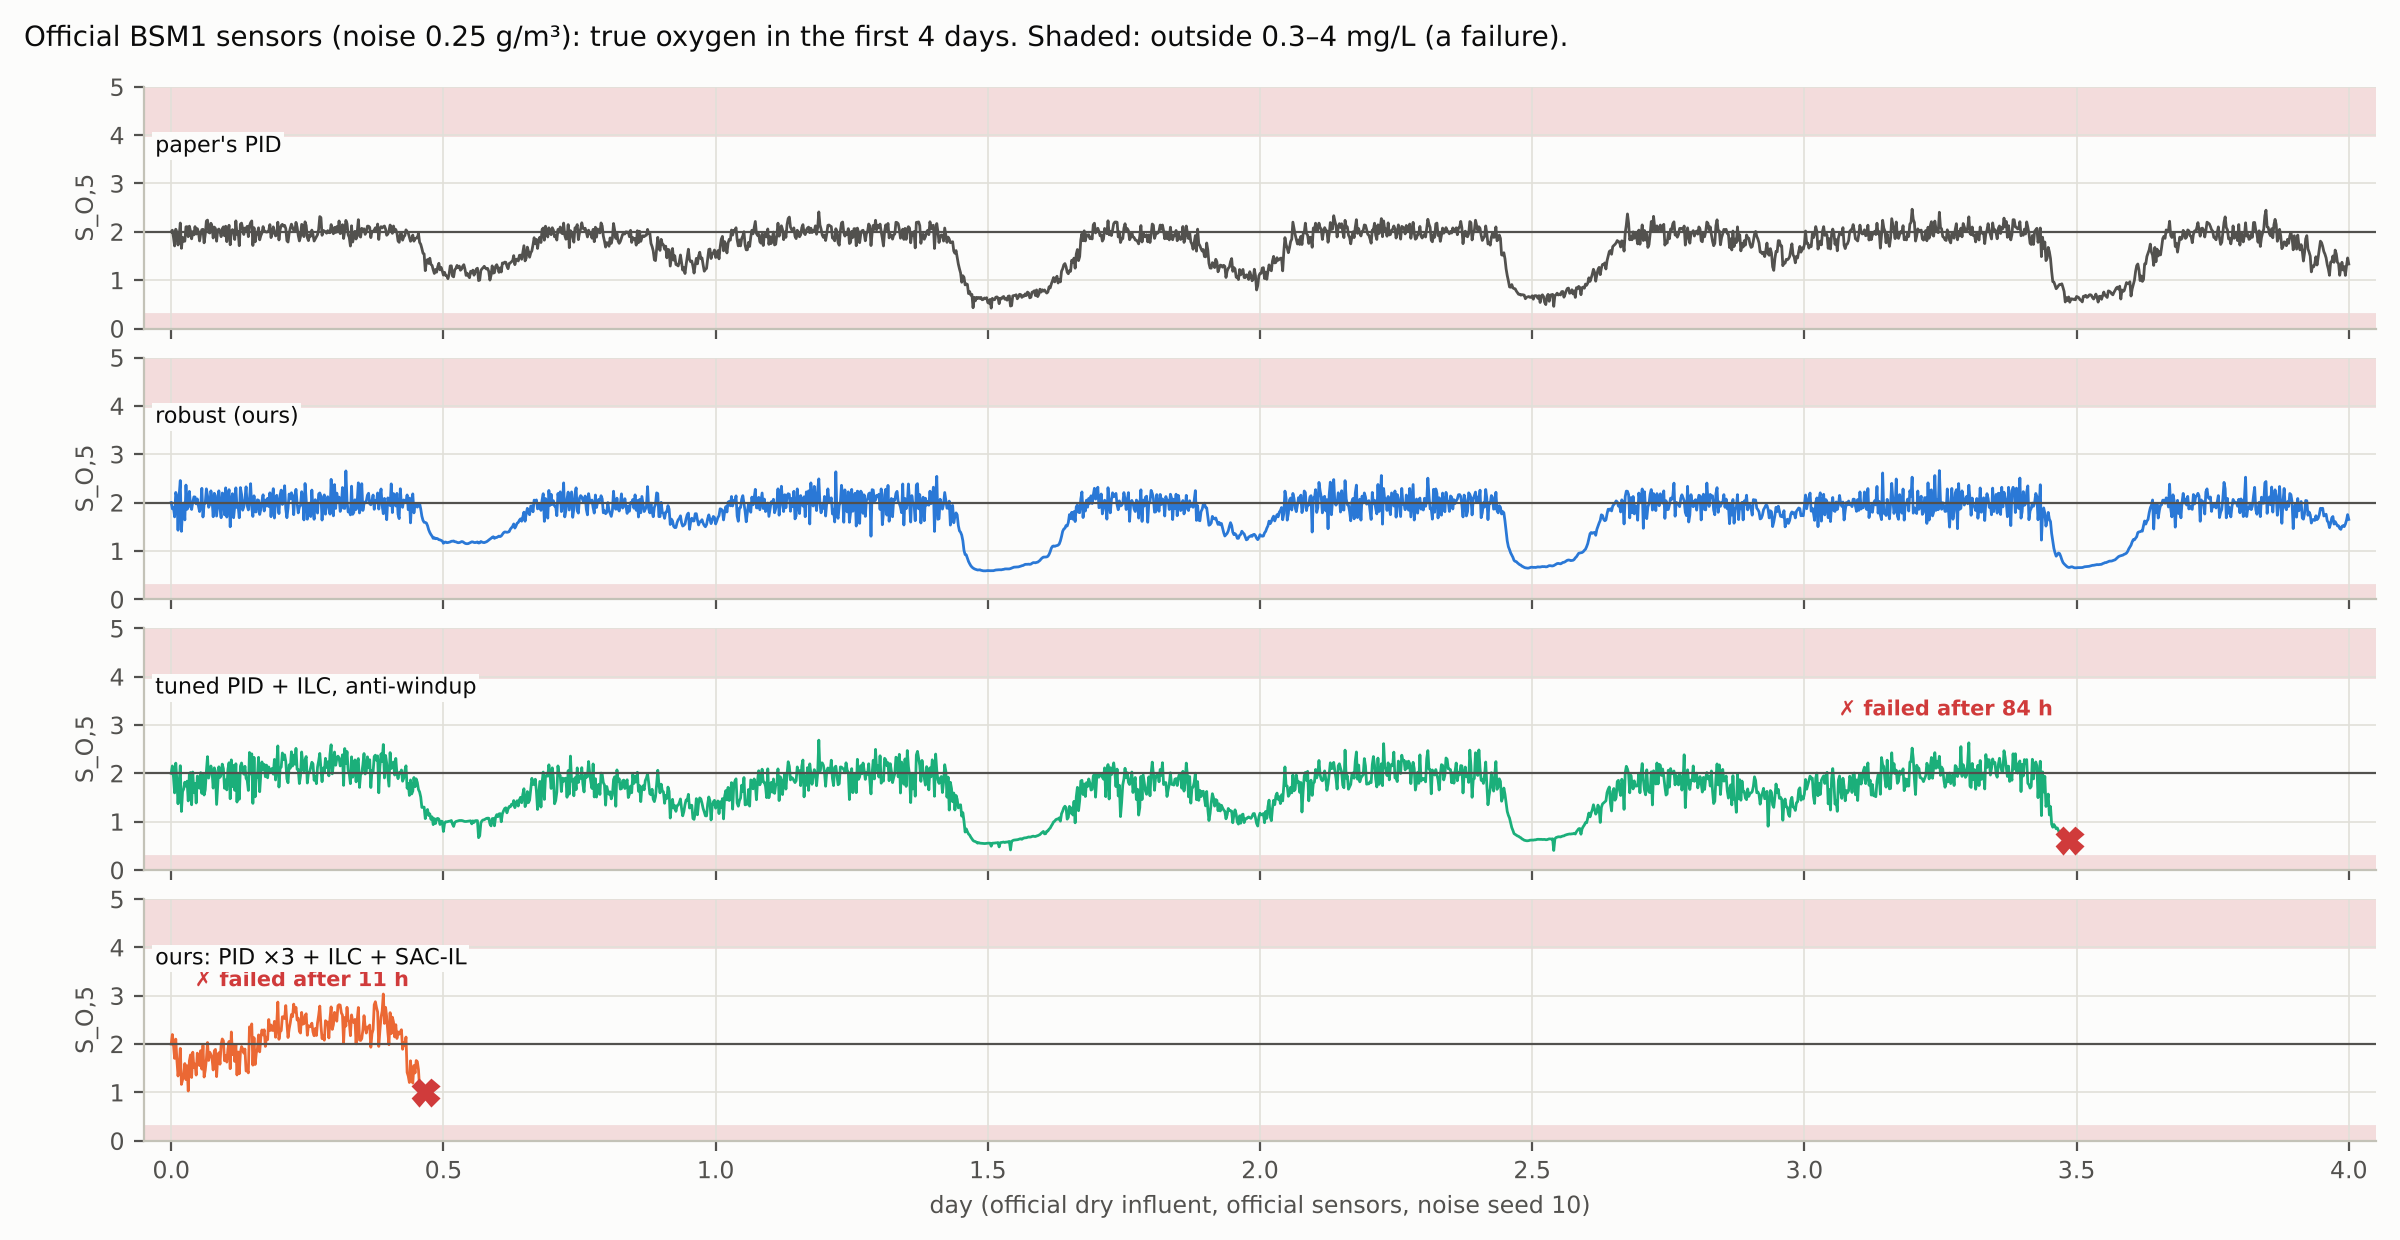
\includegraphics[width=\columnwidth]{f6_sensor_noise}
\caption{True oxygen over the first four days with the official sensors
(dry influent, noise seed 10). The paper's PID and the robust variant stay
in range; the tuned PID+ILC-AW fails after 84\,h, and PID$\times$3+ILC+SAC-IL
after 11\,h.}
\label{fig:noise}
\end{figure}

Fig.~\ref{fig:noise} shows why. With 0.25\,mg/L of measurement noise on a
2\,mg/L set point, a high-gain oxygen loop passes the noise straight to the
aeration, and the larger the gain, the larger the excursions of the true
oxygen.

\begin{figure}[!t]
\centering
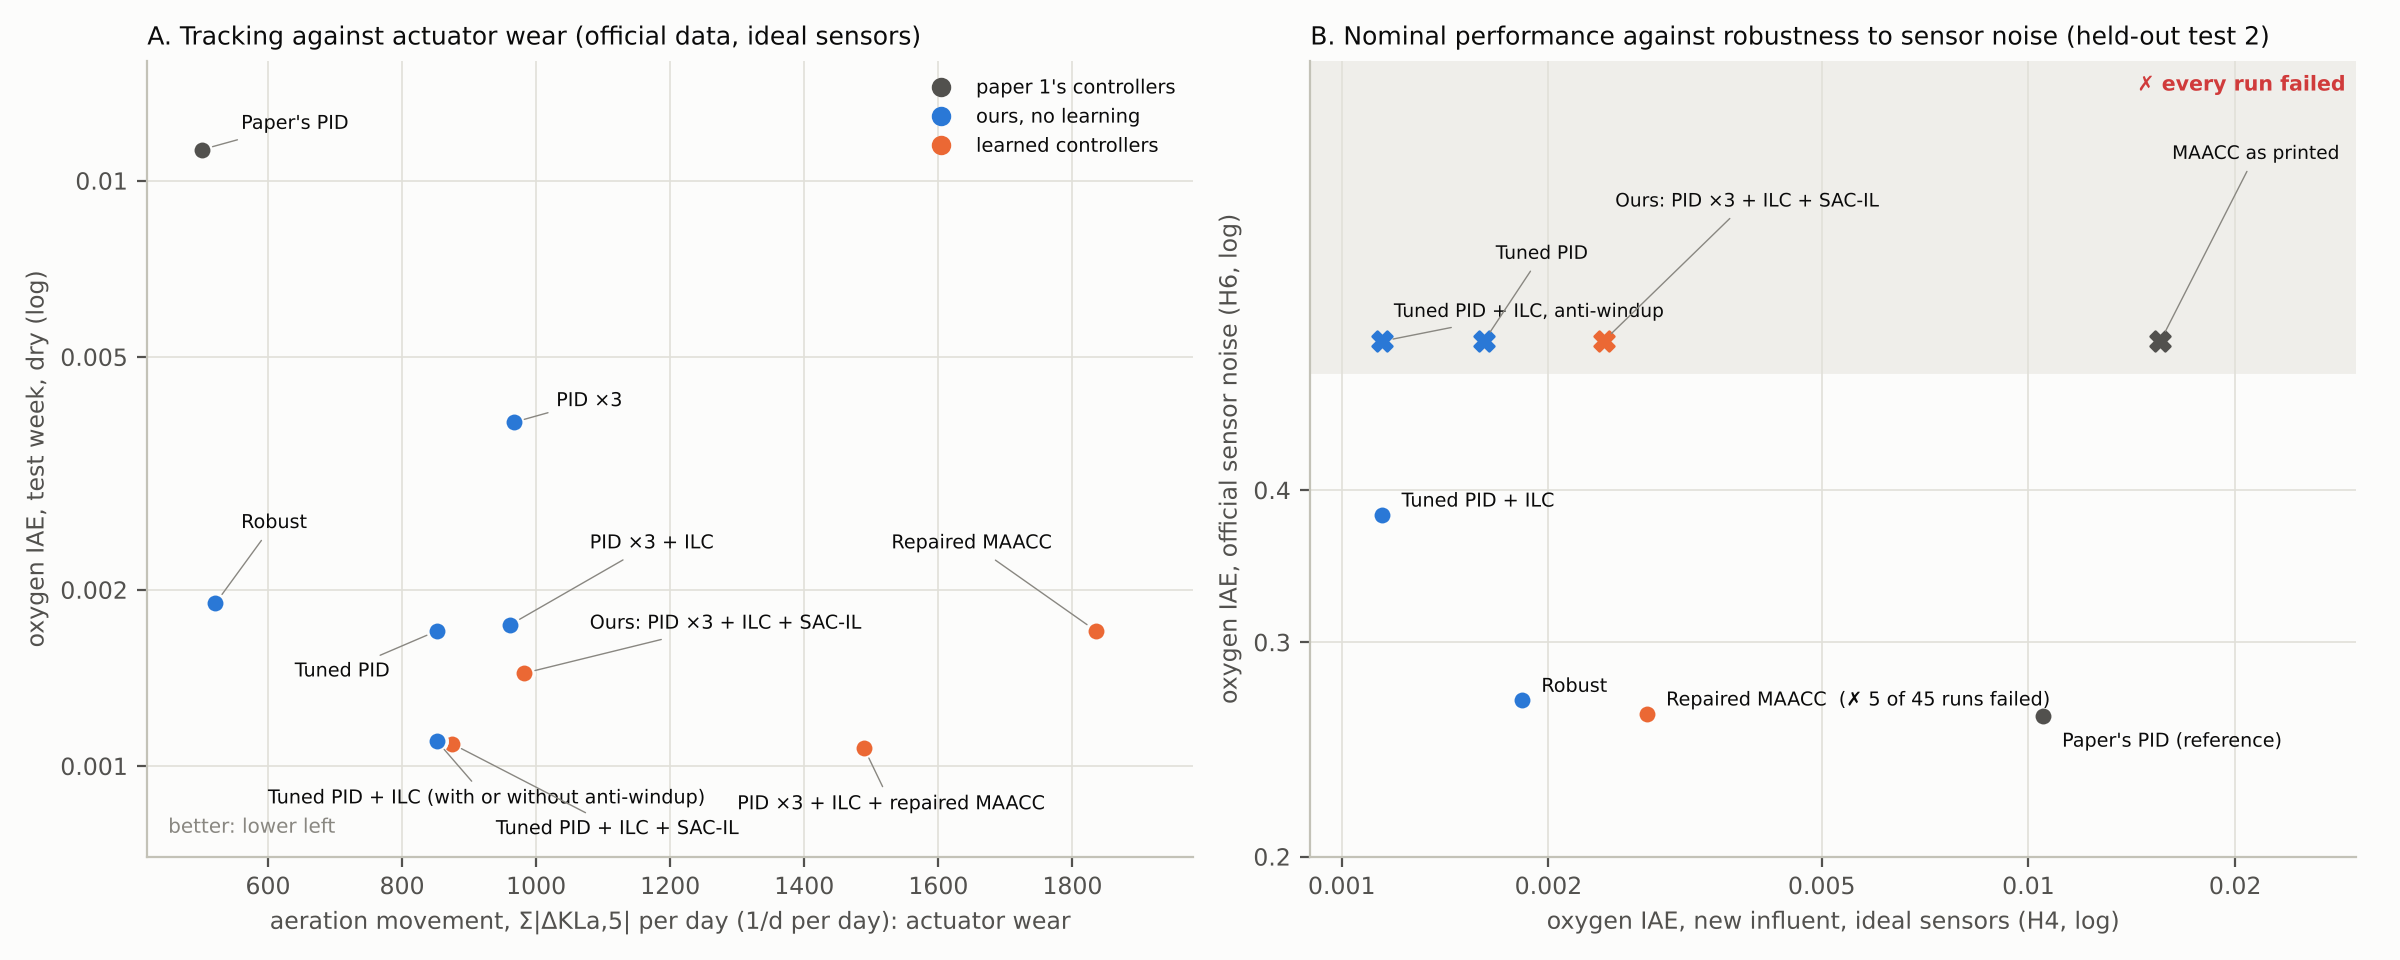
\includegraphics[width=\columnwidth]{f4_tradeoffs}
\caption{(a) Oxygen IAE against aeration movement, test week, dry. (b) Error
on new influent with ideal sensors (H4) against error with the official
sensors (H6). Controllers that are accurate without noise lose their
advantage, or fail, with it.}
\label{fig:tradeoffs}
\end{figure}

Fig.~\ref{fig:tradeoffs} puts the two sides together: accuracy with ideal
sensors and accuracy with real ones pull in different directions, and no
controller we tested is good at both.

%=====================================================================
\section{Discussion}
\label{sec:disc}
%=====================================================================

\emph{Why MAACC as printed does not learn.} An adaptive critic that updates
once per step, from that step alone, with small learning rates and a
learning signal near $10^{-4}$, cannot move far from its starting point in
the 26\,879 steps of a run. Starting from the PID makes it safe, but also makes it the
PID. Once it re-uses its data and has a stable target, the same
architecture learns. We think the gap between our runs and the published
numbers more likely lies in training details missing from the paper than in
the architecture.

\emph{Why tuning and ILC do so well.} The BSM1 influent repeats daily, and
most of the error a PID leaves is the lag behind that daily pattern. An ILC
is built for exactly this and needs no model, no training data and about a
microsecond per step. A learned correction on top has little left to
correct. We would ask of any learned controller on BSM1 that it be compared
with a tuned PID with a daily feedforward, not only with a fixed PID.

\emph{Why the held-out tests matter.} On the nominal test, the ranking of
our controllers is clear and stable across seeds. Two realistic changes,
a different influent and the benchmark's own sensor models, reversed most
of it. A controller that fails within half a day under the official sensor
noise would not be usable on a plant, however it scores with ideal sensors.
That the paper's comparatively low-gain PID survives this test best is
consistent with standard PID practice~\cite{astrom2006pid}: gain bought on
an ideal measurement is paid for with noise.

\emph{Recommendations.} From this study we would ask four things of any
learned controller evaluated on BSM1:
\begin{enumerate}
\item compare it with a PID tuned under a stated rule and with a daily
  feedforward such as the ILC, not only with a fixed PID;
\item report results with the official sensor models switched on, and on
  influent not used for tuning or training;
\item report actuator movement and failures next to the tracking error;
\item fix the test protocol before the test is run, and publish it.
\end{enumerate}

\emph{Cost.} Every controller here runs far faster than the 45-s period:
5\,$\mu$s per step for the PID, 37\,$\mu$s for MAACC, 35\,$\mu$s
for the SAC actor and about 1\,$\mu$s for the ILC. SAC-IL needs a week of
recorded expert data and about a quarter of an hour of training per run.
The tuned PID costs 36 short simulations per loop.

%=====================================================================
\section{Limitations}
%=====================================================================

\begin{itemize}
\item All percentages are against our reimplementation of the paper's PID,
  which matches the published oxygen error but not the nitrate error.
\item The failure rule, the $S_I$ correction, the train/test split, the
  clarifier stand-in for BSM2 influent and the sensor-noise generator (a
  seeded draw every 45\,s; the official model reads a 1-min noise file)
  are our choices.
\item PID controllers are deterministic and were run once per case; learned
  controllers have five training runs. With 6 windows or 9 noise runs per
  held-out condition we report means, counts and ``better in $k$ of $n$'',
  but no confidence intervals or significance tests.
\item The test week was looked at before the round of changes that
  introduced the bumpless update, dropped the nitrate ILC and added the
  tuned PID, so for those changes it is not fully unseen. Only the held-out
  tests were fixed before they were run.
\item Re-running a stored controller is exact. Retraining on another
  machine gives results near, not equal to, ours.
\item We studied one paper's controller in depth. The other two learned
  controllers of this line of work~\cite{du2023do,zhao2025ioql} were
  reimplemented but are not reported here.
\end{itemize}

%=====================================================================
\section{Conclusion}
%=====================================================================

MAACC as printed does not learn on the official BSM1, but with repaired
training its architecture does. On the standard nominal test, however, a
carefully tuned PID with a daily iterative learning controller is as good as
any learned controller we tried, and adding SAC-IL to it changes nothing.
Two pre-registered held-out tests showed that the official sensor noise
is the real constraint: every high-gain controller lost its advantage or
failed, and none beat the paper's PID there. The recommendations in
Section~\ref{sec:disc} follow from this. The open problem it leaves is a
controller that is both accurate and robust to realistic measurement noise.

%=====================================================================
\section*{Code and Data Availability}
%=====================================================================
The code, all result files, the figures, the audit script and the
held-out protocols are at
\url{https://github.com/Amritha902/water_resource}. The protocols were
pushed in commits \texttt{72d1d14} (test~1), \texttt{f1245d2} (amendment),
\texttt{22b53fa} (frozen controllers) and \texttt{378ac3d} (test~2), each
before the first run of its test. \texttt{experiments/46\_paper1\_audit.py}
re-runs the audit.

\section*{Acknowledgment}
\fillin{Thank your supervisor, institution and any funding source here.}

\fillin{AI-assistance disclosure. Check your target venue's policy and state
here, in your own words, which tools you used and for what (for example
code, analysis, figures or text drafting). Remove this note once done.}

\bibliographystyle{IEEEtran}
\bibliography{refs}

\end{document}
